%% LyX 2.0.5.1 created this file.  For more info, see http://www.lyx.org/.
%% Do not edit unless you really know what you are doing.
\documentclass[12pt,english]{report}
\usepackage{mathptmx}
\renewcommand{\familydefault}{\rmdefault}
\usepackage[T1]{fontenc}
\usepackage[latin9]{inputenc}
\usepackage[a4paper]{geometry}
\setcounter{secnumdepth}{2} % Changed from 3 to 2. 0-chapter 1-section 2-subsection 
\setcounter{tocdepth}{2} % Changed from 3 to 2. 0-chapter 1-section 2-subsection 
\setlength{\parskip}{\medskipamount}
\setlength{\parindent}{0pt}
\usepackage{verbatim}
\usepackage{pdfpages}
\usepackage{graphicx}
\usepackage{subfig} %% This package has to be here
\usepackage{setspace}
\usepackage{arabtex}
\usepackage[numbers]{natbib}
\usepackage{nomencl}
\usepackage{amsthm}
\usepackage{amsmath}
\usepackage{amsfonts}


\usepackage{etoolbox}
\newtoggle{edit-mode}
%\togglefalse{edit-mode}  
\toggletrue{edit-mode}
\iftoggle{edit-mode}{
\geometry{verbose,tmargin=2cm,bmargin=2cm,lmargin=2cm,rmargin=6cm,headheight=1cm,headsep=1cm,footskip=1cm, marginparwidth=5cm}
}{
\geometry{verbose,tmargin=2cm,bmargin=2cm,lmargin=2cm,rmargin=2cm,headheight=1cm,headsep=1cm,footskip=1cm}
}

\makenomenclature

% Theorem Styles
\newtheorem{theorem}{Theorem}[section]
% Definition Styles
%\theoremstyle{definition}
\newtheorem{definition}{Definition}[section]
\newtheorem{example}{Example}[section]
\theoremstyle{remark}
\newtheorem{remark}{Remark}

\usepackage[linesnumbered]{algorithm2e}

\begin{document}
\printnomenclature{}

\tableofcontents{}

\chapter{Handwritten Arabic Recognition}

\section{Introduction}

\iftoggle{edit-mode}{\hspace{0pt}\marginpar{Complexity of the Arabic handwriting recognition}}{}
On-line handwriting recognition is one of the very complex and challenging problems in the pattern recognition field due to the variability of writing styles, cursive writing, text size differences and sampling issues caused by duplicate samples resulted from hesitate writers as well as non-adjacent consecutive samples caused by fast writers \cite{verma2004feature}. The problem that makes the recognition of on-line handwriting recognition difficult is variation of shapes of the characters resulting from writing habits, styles, and the social and educational level of the writer.
%Correct and precise classification is a fundamental part of any \emph{Optical character recognition} (OCR) system.
In this chapter we will discuss theoretical aspect as well as implementation details of the classification engine implemented in our system. \emph{TODO: fix this paragraph}\\ 

\iftoggle{edit-mode}{\hspace{0pt}\marginpar{Input-output}}{}
Given a stroke sequence, and a position as an input parameter to the classifier, it produces a list of candidate samples from the sample set which are most similar to the given sequence, with a scoring attached to each candidate. Thus, actually, the classifier contains four databases. On for each letter position. This partitioning of the samples to four database, clearly, improve the classification power and the accuracy of the classification and scoring.\\

\iftoggle{edit-mode}{\hspace{0pt}\marginpar{Performance}}{}
The performance of the on-line classifier is a crucial property of the 
needed classifier since, as mentioned in the overview in chapter \ref{}, the goal of the system is to perform strokes segmentation and letters recognition while the stroke is being written.\\ 

\iftoggle{edit-mode}{\hspace{0pt}\marginpar{Constructs classification}}{}
In the on-line text recognition, the classification can be done in several levels. The Recognition system can be built to classify an entire words, Word-parts, letters or even strokes. In this work we chose to work with strokes, since it represent the most basic element a writer can produce after the point, and it contains in most cases a single letter or more.\\

\iftoggle{edit-mode}{\hspace{0pt}\marginpar{Talk in general about the technique we use - mention each stage in general}}{}
Text Recognition can be broken down into three main stages: \emph{preprocessing}, \emph{feature extraction} and \emph{classification}. The preprocessing stage usually consists of normalization, re-sampling, noise elimination and smoothing steps to give the a uniform structure and avoid irrelevant information that can negatively affect the recognition. In the feature extraction stage, important information in the data is highlighted and represented as vectors in the feature space which is used by the classifier. The last important step is classification, which identify the class for which the sample belong.\\

%We will start our discussion by giving the required background to pattern recognition, in general, and to the handwritten text recognition field in particular.\\

%\iftoggle{edit-mode}{\hspace{0pt}\marginpar{Types of learning problems.}}{}
%Machine learning is a branch in computer science of getting computers to act without being explicitly programmed. 
%The are mainly three types of learning: supervised, unsupervised and reinforcement learning.
%In the supervised learning, as seen above, a set of classified samples is given. In the unsupervised learning case, unlabeled data is given and the goal is to find a hidden structure in it. The reinforcement learning is a type of learning inspired by behaviorist psychology, concerned with how software agents ought to take actions in an environment so as to maximize some notion of cumulative reward. The handwriting recognition in most of it's implementation is a supervised learning problem.\\

\iftoggle{edit-mode}{\hspace{0pt}\marginpar{The learning problem.}}{}
In \emph{supervised learning}, classification is the problem of identifying to which of a set of classes a new observation belongs. It is done on the basis of a training set of data containing instances for which the their class membership is known.
Formally, the supervised learning problem is defined as follows:
\begin{definition}
Given a domain space $X$, a target space $Y$ and a training set $S=\{(x_i,y_i)\}_{i=1}^{m}$ where $x_1,x_2,..,x_n\in X$ and $y_1,y_2,...,y_n \in Y$. Let us assume that there is an unknown target function $f$ for which $f : X\rightarrow Y$. A Learning algorithm $A$ produces hypothesis function $h$ based on $S$ such that $h \approx f$, i.e. the function $h$ is an approximation for the target function $f$ and $h \in H$, the hypotheses set. 
\end{definition}

\begin{figure}
\centering
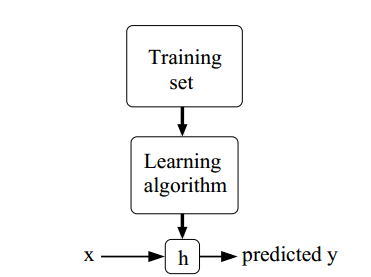
\includegraphics[width=0.5\textwidth]{./figures/machine_learning_diagram}       
\caption{A learning algorithm scheme}
\label{fig:machine_learning_diagram}
\end{figure}

\iftoggle{edit-mode}{\hspace{0pt}\marginpar{The classification problem}}{}
In many cases, the learning problem is actually a classification problem. For any given classification problem, there is an intuitive belief that there exist a space to which the samples can be transformed and in which can be portioned into regions that represent categories. Accordingly, the problem of classification is basically the problem of portioning the sample space into regions. Having done that, classifying a new unlabeled observation is done by determining the partition it belongs to. Ideally, one would like to arrange this partitioning so that none of the decisions is ever wrong. When this cannot be done, one would like to minimize the probability of error \cite{duda1973pattern}.

\iftoggle{edit-mode}{\hspace{0pt}\marginpar{What we actually try to do? and How?}}{}
Since no such partition on the raw data space is known. We try to find the mentioned space in the feature space and to approximate the mentioned partitioning.
 \emph{TODO: describe what each step do in a high level.}

\iftoggle{edit-mode}{\hspace{0pt}\marginpar{Types of approaches in the supervised Learning.}}{}
%In machine learning, pattern recognition is the assignment of a label to a given input value. 
Many supervised learning approaches and algorithms were proposed to solve the classification problem. Decision trees, artificial neural networks, support vector machines, Bayesian networks and nearest neighbor are few well-known learning techniques. A review on the supervised classification algorithms is given by Mohamed Aly in \cite{aly2005survey}.The role of the machine learning specialist is to identify the type of the learning problem and meet the needs of the problem by stitching the best solution for it. The classification process is usually contains several steps. These preliminary steps include normalization, noise removal, feature extraction, dimensionality reduction, etc. emph{[fix]}\\


\iftoggle{edit-mode}{\hspace{0pt}\marginpar{Classification techniques in HW recognition}}{}
Different approaches were considered to solve the text recognition problem. Each has it's advantages and drawbacks, and each is suitable for a certain system requirements and implementation.
The classification algorithm used in the recognition process is the most central stage. All the preprocessing stages prepare the data for the classification stage. The classification stage may be composed of more than a single stage.  
In the following, we will mention the few most common approaches commonly used for letters classification and discuss their advantages and drawbacks.\\

\iftoggle{edit-mode}{\hspace{0pt}\marginpar{HMM - An introduction}}{}
Unlike in the off-line case, on-line handwriting can be viewed as temporal series, therefore many pattern recognition techniques from the temporal information field were adopted for handwriting recognition. One example is the  \emph{hidden Markov models} (HMM). HMM is an extension of the discrete-state Markov process. \emph{TODO: give some more information about the theory of HMM}

\iftoggle{edit-mode}{\hspace{0pt}\marginpar{HMM for online handwriting recognition}}{}
There is a vast amount of studies done in the field of handwriting recognition field that use HMM \cite{pechwitz2003hmm, khorsheed2003recognising, al2007combination, benouareth2008arabic, mahmoud2008recognition, shu1996line}. 
Letters, words and sentences can be modeled using HMM and using the solution of the learning problem, letter words and sentences can be identified. Reader unfamiliar with this approach, a good introduction on using HMM for time series classification in general and text recognition in particular can be found \cite{kadous2002temporal, shu1996line}.\\ 

\iftoggle{edit-mode}{\hspace{0pt}\marginpar{HMM - disadvantages}}{}
While having many advantages, there are some drawback of using HMM, Kondous has pointed out in his Ph.D Thesis \cite{kadous2002temporal}. First, it makes powerful assumption about the data that may not necessarily true. One example is the Markovian assumption, i.e., that the transition probabilities depend only on the current state. Second, there is no specific way to determine the number of states, thus intelligent guesses and try and error are usually employed. Furthermore, the states and transitions depend on the class being learned. For example, is there any reason why the words "dog" and "butterfly" would have similar states and transitions? Third, HMM requires a very large amount of data for its training.\\

\iftoggle{edit-mode}{\hspace{0pt}\marginpar{Artificial Neural Networks - an introduction}}{}
Artificial neural network is also a widely used technique for letters recognition. It is a generalization of linear discrimination. 

\iftoggle{edit-mode}{\hspace{0pt}\marginpar{ANN - drawbacks}}{}


\iftoggle{edit-mode}{\hspace{0pt}\marginpar{k-NN classifier in general}}{}
The k-nearest neighbors algorithm (k-NN) is a well-known classification technique in supervised learning. It predicts the query objects class memberships based on the k closest training examples. The k-nearest neighbor algorithm is one of the simplest of all machine learning algorithms: an object is classified by a majority vote of its neighbors, with the object being assigned to the class most common amongst its k nearest neighbors (k is a positive integer, typically small). If $k=1$, then the object is simply assigned to the class of that single nearest neighbor. In many cases the notion of similarity between sample object is obvious, however in many other interesting cases the distance between objects cannot be easily defined.
Beside its simplicity, k-NN has some major advantages. First, k-NN is a good learning method for complex target functions. Second, it is easy to implement. Third, arbitrary objects similarity function can be applied easily.\\

\iftoggle{edit-mode}{\hspace{0pt}\marginpar{Advantages and Downside of the k-NN classifier}}{}
k-NN algorithm has dome drawbacks that reader needs to note. k-NN needs a large data set in-order to achieve high classification accuracy. Another drawback is that it is very sensitive to data errors and can be easily fooled by outliers.\\

\iftoggle{edit-mode}{\hspace{0pt}\marginpar{Scoring-based NN classification}}{}
Several machine learning problems, especially those having a large number of classes, the classifier, returns a set of potential candidate classes or even specific samples in the. In these cases, for each candidate class, the classifier usually gives a scoring that can be used by a later part in the classification process (e.g. in the post processing). Such approach is taken for objects classification in our system. sample set that are closely resembles a given unknown sample. This approach can be used for both supervised and unsupervised learning domain. In the supervised learning case since the classification of the returned samples is known, the hypothesis function, classifies the inputed sample based of candidate labels.\\

\iftoggle{edit-mode}{\hspace{0pt}\marginpar{Why did we use the NN as a classifier}}{}
For the disadvantages for HMM and NN techniques mentioned above and the intuitive and simplicity of the and for my personal interest in similarity measure techniques that can be integrated classifier, we have chosen to use Nearest Neighbor classifier classification.\\ 

\iftoggle{edit-mode}{\hspace{0pt}\marginpar{NN classification}}{}
In the k-NN problem a set of data points in d-dimensional space is given and for a query point q, the nearest or generally k nearest points of P to q can be reported efficiently. The distance between two points can be defined in many ways as will be detailed in section \ref{[]}.k-NN based classification a very basic and common approach for implementing the pattern classification. However, the retrieval of the exact k-Nearest Neighbors for a given query object $q$ and a database of sample set $S$ suffers from bad performance that is mainly caused by two factors. The first, is the total numbers of samples in the data. This issue will be discussed in Section \ref{sec:similarity_search} and the other is the dimensionality of objects in the data (known as the \emph{curse of dimensionality}). Computing exact nearest neighbors in dimensions much higher than 8 seems to be a very difficult task. However, the first issue has much smaller impact on the speed of the nearest neighbor retrieval and can be healed easily by using dimensionality reduction techniques which will be discussed in details in Section \ref{sec:dimensionality_reduction}. However, the first issue, i.e., the size of the sample data, is crucial. The simplest solution to the NN problem is to linearly go over the entire sample set and keep track of the best k best nominates so far. The running time of this algorithm in $O(Nd)$ where $N$ is the cardinality of sample set and d is the dimensionality of the sample set. While looking in the entire database for the kNN is not permissible for most applications. The only advantage of this approach is that it requires no extra space, beyond the amount of the memory needed for keeping the sample set. This issue is will be treated in Section \ref{similarity_search}. \\

\emph{TODO: show a diagram of the letters learning process}

\emph{TODO: show a diagram of substrokes clasgmssification process.}


%%%%%%%%%%%%%%%%%%%%%%%%%%%%%%%%%%%%%%%%%%%%%%%%%%%%%%%
\newpage{}
%%%%%%%%%%%%%%%%%%%%%%%%%%%%%%%%%%%%%%%%%%%%%%%%%%%%%%%

\section{Samples Preprocessing}

The data obtained by the digitizer is composed of points in the plane that represent the trajectory scribed by the writing instrument on the tablet surface. Usually, samples are taken in time intervals, thus slow pen motion regions are oversampled and fast motion regions are under-sampled. In addition, when such devices are used to capture handwriting strokes, the shapes of the strokes present a jagged form and the obtained data is non-uniform and noisy. Further imperfections are caused by hand vibrations and duplicated sampled points resulted from hesitant writing. This noise should be reduced as much as possible since it influence the further processes, such as feature extraction and classification \cite{al2011online} \cite{huang2009preprocessing}.  
To overcome the flaws mentioned, preprocessing operations are usually applied. The preprocessing steps imposes certain uniform structure on the data to comply with the input structure required by the latter parts of the system, such that vector length, sequence bounds, etc.\\

\emph{TODO: mention other preprocessing approaches mentioned in the literature, like rotation normalization, slant normalization, and missing points interpolation. see \cite{jaeger2001online}.}

As seen in figure \ref{[]} and \ref{[]}, preprocessing is performed in both letters learning and classification of strokes.
Preprocessing is also done in the segmentation phase, however, not all steps mentioned in this section are performed. For more information see section \ref{[]}

Data samples must be of the same dimension for the system to work properly. Since the collected letters in the database are of varying sizes, they were all resized to some standard size. and re-sampled to to achieve same length sequences.
Our preprocessing phase include three steps in the following order: \emph{Normalization and Translation}, \emph{Noise Elimination} and then \emph{Smoothing and Re-sampling}.\\ 

In figure \ref{fig:D_before_after_preprocessing} we show a sample of the letter \RL{d} sequence before and after preprocessing.\\ 

In the next sub-sections we will describe in details each part of the preprocessing procedure.

\begin{figure}
	\centering
        \subfloat[]{
            \label{fig:letter_before_preprocessing}
            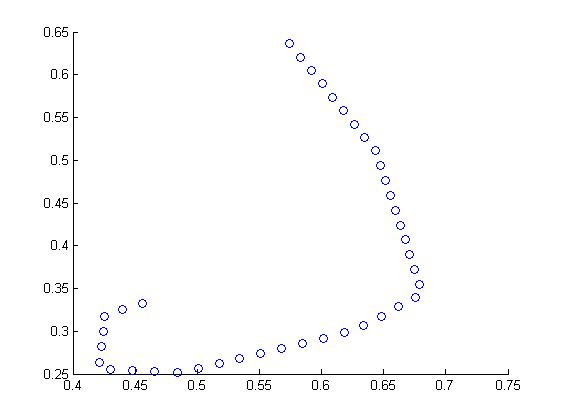
\includegraphics[width=0.5\textwidth]{./figures/letter_before_preprocessing}
        }
        \subfloat[]{
           \label{fig:letter_after_preprocessing}
           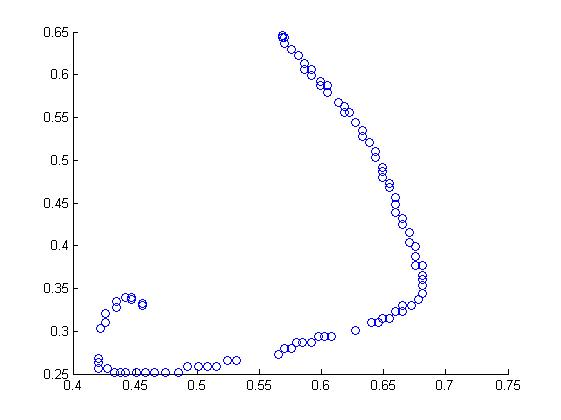
\includegraphics[width=0.5\textwidth]{./figures/letter_after_preprocessing}
        }        
    \caption{The letter \RL{d} before (a) and after (b) preprocessing}
   \label{fig:D_before_after_preprocessing}
\end{figure}

\emph{refer to the slant and Rotation normalization, i.e. why we don't do it. Is slant common in Arabic?
}

\subsection{Normalization and Translation}

Size normalization is done to achieve a uniform size of the bounding box surrounding the pattern. This is done to enable the classifier to recognize the sequence pattern even when the stroke is written in different sizes. Shape similarity algorithms tend to be sensitive for non-uniform shapes size, thus this procedure is important and can be found in many approaches in the literature. 
However, this method could not be applied since normalization is done in our system on the stroke level which could contain a letter, at least.
In our approach size normalization was applied on each stroke such that all strokes have $[0,1]\times[0,1]$ bounding box but retain their original aspect ratio. We include in this step also translation of the sequence's center of gravity to the origin point $[0,0]$.
Given the stroke sequence $S=\{p_i\}_{i=1}^{n}$, the normalized sequence $\bar{S}=\{\bar{p_i}\}_{i=1}^{n}$ is calculated by: 

\begin{equation}
{\bar x_i} = {{\left( {{x_i} - {\mu _x}} \right)} \over W},{\bar y_i} = {{\left( {{y_i} - {\mu _y}} \right)} \over W}
\end{equation}
Where
\begin{equation}
\mu  = \left( {{\mu _x},{\mu _y}} \right) = \left( {{1 \over N}\sum\limits_{i = 1}^N {{x_i}} ,{1 \over N}\sum\limits_{i = 1}^N {{y_i}} } \right)
\end{equation}
\begin{equation}
W = \max \left( {{d_x},{d_y}} \right)
\end{equation}
\begin{equation}
{d_x} = {x_{\max }} - {x_{\min }};\,\,\,{d_y} = {y_{\max }} - {y_{\min }}
\end{equation}
\begin{equation}
{x_{\max }} = \mathop {\max }\limits_i \left( {{x_i}} \right),\,\,{x_{\min }} = \mathop {\min }\limits_i \left( {{x_i}} \right),\,\,{y_{\min }} = \mathop {\min }\limits_i \left( {{y_i}} \right),\,\,{y_{\min }} = \mathop {\min }\limits_i \left( {{y_i}} \right)
\end{equation}  

\subsection{Noise Elimination}
The input obtained by the digitizer may contain a large amount of noise which is mainly duplication of points. In this process redundant points are filtered out and a similar sequence with fewer points is obtained.
In order to eliminate redundant points irrelevant for pattern classification and screening out unwanted noise and vibrations in the letter inscription we have used the \emph{Douglas-Peucker Polyline Simplification algorithm} described in \cite{douglas1973algorithms}. Briefly, it is a line simplification algorithm to reduce the number of vertices in a piecewise linear curve according to a specified tolerance. The algorithm is also known as \emph{Iterative Endpoint Fit}. The resulted curve is a skeletonized angular sequence. The Normalization is done before the Simplification, since we need a constant simplification parameter $\varepsilon$ which was tuned for $1\times1$ bounds. 
Assuming the stroke presentation is a sequence of points $S$, the sensitivity parameter that was used in our work is:
\begin{equation}
\varepsilon  = {1 \over {200}}\sqrt {{d_x}^2 + {d_y}^2}
\end{equation}

\begin{figure}
\centering
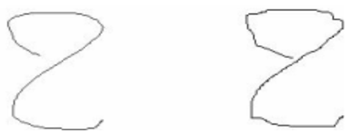
\includegraphics[width=0.7\textwidth]{./figures/ha_simplification}       
\caption{Non Simplified representation of the letter \RL{.h} (Ha) is shown on the right. A simplified version is shown on the left. \emph{TODO: change the pictures to something better}}
\label{fig:ha_simplification}
\end{figure}

\subsection{Smoothing and Re-sampling}
As a result of the simplification process the points are not distributed uniformly along the stroke trajectory. Naturally, there are less point in relatively straight areas and a higher amount of points in the curved areas of the stroke.\\ 
%if we wont use simplification we can write this: The re-sampling is needed to prevent the unbalanced sampling density, which may be influenced by the sampling rate and the user non-uniform letter drawing. 
The re-sampling produces equidistant smoothed data sequence. 
The Re-sampling is performed using splines interpolation as follows:\\
Given a stroke $S=\{p_i\}_{i=1}^{n}$ and the re-sampling target number $R$, let $\{X(a_i)\}_{i=1}^{n}$ and $\{Y(a_i)\}_{i=1}^{n}$ represent the x-axis and the y-axis sequences with respect to the parameter $a_i$ which is defined as follows:

\begin{equation}
a_i=a_{i-1}+arclen(p_{i-1},p_i) 
\end{equation}  

\begin{equation}
X(a_i)=x_i 
\end{equation}  

The arc-length of the stroke is given by $L=a_n$.\\

A piecewise linear interpolations $q_X(a)$ and $q_X(a)$ are created for the $X$ sequence and $Y$ sequence respectively.
The breaks are the $a_i$ sequence and the coefficient of the linear polynomial are $\alpha_{i} = \frac{X(a_i)-X(a_{i-1})}{a_{i}-a_{i-1}}$ 

\emph{[we use quadratic splines for smoothing and simplification.]}

let $t_i=i\frac{L}{R}$ for $i=0,...,R$.
The re-sampled sequence is given as follows:
\begin{equation}
\widehat{S}=\{(q_X(t_i),q_Y(t_i))\}_{i=1}^{R}
\end{equation}

The target number of points is set to 40. We had to find a number that is good enough for both long and short strokes since strokes can span over a single letter or a whole WP.

\emph{[TODO: show the following images: 1. the scattered stroke, 2. X and Y as a function of t., 3. X and Y resampledm and 3. the stroke resampled. ]}

\emph{[TODO: talk about splines.]}

\emph{TODO: talk about the other smoothing techniques as described in \cite{jaeger2001online} -- Online handwriting recognition: the NPen++ recognizer}

\subsubsection{Approach 1 - Using piecewise linear interpolations}

\subsubsection{Approach 2 - Using quadratic splines}

\begin{figure}
\centering
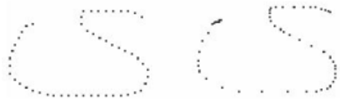
\includegraphics{./figures/y_resampling}       
\caption{Representation of a non-resamples sequence of the letter \RL{y} (Y) is shown in the right. The re-sampled version is shown on the left.}
\label{fig:y_resampling}
\end{figure}

Answer the following:
\begin{itemize}
\item Mention that the data in the database was not in the same length therefore normalziation and re-sampling were needed. 
\item Where preprocessing is used in our system? Letters Learning and strokes classification
\item What parameters were used for each preprocessing stage and why.
\item what alternatives were considered.
\end{itemize}

%%%%%%%%%%%%%%%%%%%%%%%%%%%%%%%%%%%%%%%%%%%%%%%%%%%%%%%
\newpage{}
%%%%%%%%%%%%%%%%%%%%%%%%%%%%%%%%%%%%%%%%%%%%%%%%%%%%%%%

\section{Features Extraction}
\label{sec:feature_extraction}

\iftoggle{edit-mode}{\hspace{0pt}\marginpar{Introduction}}{}
Feature extraction is certainly one of the important parts of any pattern classification system and plays an important role in the overall process of handwriting recognition. It aims is to cull informative parameters for learning and recognition of patterns.  Most classification methods require that patterns be represented in a fixed dimensional feature space that is often incompatible with input data. Poor feature extraction and selection will always result in a poor system performance, regardless of the ingeniousness of the learning and classification algorithms \cite{parizeau2001character}.\\

\iftoggle{edit-mode}{\hspace{0pt}\marginpar{Introduction - Cont.}}{}
Feature extraction methods operate differently in different domains and may have slightly different goals in different pattern recognition fields. For instance, in the image retrieval field, the input data (i.e., the image) is too large and suspected to be redundant. In this case, feature extraction techniques are used to reduce the representation of the input data into a compact representation set of features. However, In the shape recognition domain, the input data is compact and feature extraction techniques are used to transform it into feature vectors, which are usually referred to as \emph{shape descriptors}. Shape descriptors offer discriminative characterization to capture the perceptual dissimilarity between two shapes. Unlike the first case, the raw amount of data contained in feature vector usually exceeds the amount of data in the original input data.\\

\iftoggle{edit-mode}{\hspace{0pt}\marginpar{Shape Descriptors}}{}
The goal of a shape descriptor is to be able to effectively find perceptually similar shapes from a database. Shape descriptors are usually in the form of vectors that are produced to represent a given shape feature and attempts to quantify perceptual similarities between shapes. That is to say, shapes which are found perceptually similar by human have resembling descriptor than from shapes that are different from the others. Effective shape descriptor must present some essential properties such as translation, rotation and scale invariance. It also must be as robust as possible against noise so that variously distorted shapes which are tolerated by human beings when comparing shapes should be endured also by the shape descriptor. This is known as the robustness requirement \cite{zhang2004review}.\\

\iftoggle{edit-mode}{\hspace{0pt}\marginpar{Shape Descriptors properties}}{}
The following are properties of a desirable shape descriptor: 1. good retrieval accuracy; 2. compact features; 3. low computation complexity; 4. robust retrieval performance \cite{kim2000region}.\\

\iftoggle{edit-mode}{\hspace{0pt}\marginpar{Shape Descriptors - Handwriting recognition}}{}
Many shape descriptors have been developed in order to improve the segmentation and recognition rates. There are many different classifications and sub-classifications of shape descriptors according to their method of operation. The most common classification is the classification for local and global descriptors. Local descriptors calculate some feature at each sample point. An example for a local feature is the vector that contain the tangent slope angle for every given point in the sample point. \emph{Normalized curvature} and \emph{Ratio of tangent} \cite{hu1995invariant, hu1996hmm} are examples of more complex local shape descriptor. Descriptors such as cusps, crossings and loops are referred to as global descriptors and are calculated on the entire shape \cite{hu1997combining}. For a comprehensive review on shape descriptors see \cite{zhang2004review} and \cite{yang2008survey}.

%\emph{TODO: review "Local vs. global Features" (p. 30) in \cite{connell2000online} }

\iftoggle{edit-mode}{\hspace{0pt}\marginpar{Using off-line shape descriptors for on-line handwriting recognition}}{}
Many of the well known and powerful features operate on the shape's contour. This is because many descriptors were developed for off-line handwriting recognition. However, the input data in the on-line case is a sequence of points and no contour is involved. Using features in on-line handwriting recognition that we originally developed for the off-line case is common. Saabne and El-Sanna employed the \emph{Shape Context} (SC) descriptor, a global shape descriptor that was originally developed for contour based shapes,  on-line handwriting recognition in \cite{saabni2009hierarchical}. Multi Scale shape context is used by Hu and Zanibbi in \cite{husegmenting} for on-line handwritten mathematical expressions segmentation. The original definition of the mentioned features is given on the contour of the shape. However to use it in the on-line writing recognition case, the features are applied upon the stroke sequence.\\ 

\iftoggle{edit-mode}{\hspace{0pt}\marginpar{Selected Descriptors}}{}
In this work we have chosen to work with two shape descriptors, the Shape context descriptor, MAD and  the tangent angle feature. The reason for this choice is that we wanted to investigate how both global and local features effectiveness in our proposed process. More information about these features are given below.\\

\nomenclature{$SC$}{Shape Context Descriptor}
\iftoggle{edit-mode}{\hspace{0pt}\marginpar{Shape Context}}{}
Belongie and Malik have presented a point matching approach named Shape Context \cite{belongie2002shape}. The Shape context is a shape matching approach that intended to be a way of describing shapes that allows for measuring shape similarity and the recovering of point correspondences. This approach is based on the following descriptor: Pick $n$ points on the shape's contour, for each point ${p_i}$ on the shape, consider the $n - 1$ other points and calculate the coarse histogram of the relative coordinates. Equation \ref{eq:sc_bins} is defined to be the shape context of ${p_i}$.

\begin{equation}
{h_i}(k) = \# \{q \ne p_i:(q - p_i) \in bin(k) \}
\label{eq:sc_bins}
\end{equation}

The bins are normally taken to be uniform log-polar space making the descriptor more sensitive to positions of nearby sample points than to those of points farther away. This distribution over relative positions is robust and compact, yet highly discriminative descriptor. The basic Idea of the Shape Context Descriptor is illustrated in Figure \ref{fig:shape_context_demo}. This can be calculated in $O(N^3)$ time using the Hungarian method. \\

\begin{figure}
\centering
\subfloat[]{
    \label{fig:shape_context_offline}
    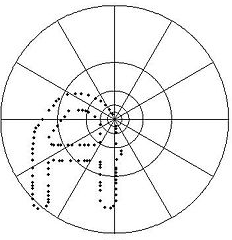
\includegraphics[width=0.27\textwidth]{./figures/shape_context_offline}
}
\subfloat[]{
	\label{fig:shape_context_online}
     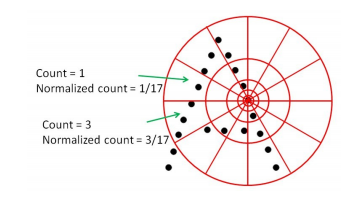
\includegraphics[width=0.3\textwidth]{./figures/shape_context_online}
}        
\caption{Diagram of the log-polar bins used to compute the shape context. On-line and off-line}
\label{fig:shape_context_demo}
\end{figure}

\nomenclature{MAD}{Multi Angular Descriptor}
\iftoggle{edit-mode}{\hspace{0pt}\marginpar{MAD}}{}
The other shape descriptor used in this thesis is the Multi Angular Descriptor (MAD).
MAD was proposed by Saabni in \cite{saabni2013multi}. It captures the angular view to multi resolution rings in different heights. The shape is treated as a two dimensional set of points and the different rings are upper view points from rings around the shape centroid with different sizes and heights. To enables scale and translation invariance, the sizes and heights of these rings are calculated using the diameter and centroid of the shape.
Formally, let $S$ be a shape and Let $C$ and $D$ be the centroid and the diameter of the shape respectively. Let $P = \{p_i\}_{i = 1}^l$ a set of $l$ point taken uniformly from the extracted contour of $S$. Given a view point $V_j$ from a given ring with height $h$ over the shape, the angle, obtained by connecting the point ${p_i} \in P$ with each point   and the plain of the shape is a rich description of the shape from this view point. Let $R$ be a ring with the radius $r$ and the center $C$ positioned above the shape $S$ with the height $h$. Let $V = \{V_i\}_{i = 1}^n$ be a set of $n$ viewpoints lying uniformly on the ring $R$ and $\alpha(V_{ij})$ to be the angle between the segment $\overline {{V_i}{p_j}}$ and the plain contains the shape $S$. The vector $Ve{c_i} = \left\{ {\alpha \left( {{V_{ij}}} \right)} \right\}_{j = 1}^l$ can be seen as watching the shape $S$ from one upper view point $V_i$. Illustration can be seen in Figure \ref{fig:mad_demo}.\\

\begin{figure}
\centering
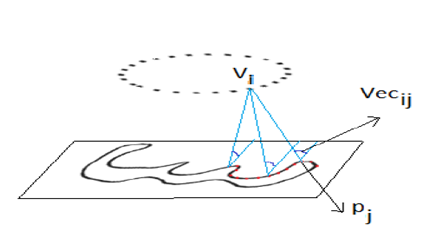
\includegraphics[width=0.5\textwidth]{./figures/mad_demo}       
\caption{In this figure we can see an example of three line segments drawn from the same viewpoint $V_i$, generating the three angles $Vec_{ij}$ with the plane of the shape. When the parameter $j$ goes over all contour points we get the vector $Vec_i$ describing the shape from the view point $V_i$ with the parameter $i$ goes over all viewpoints.}
\label{fig:mad_demo}
\end{figure}

\iftoggle{edit-mode}{\hspace{0pt}\marginpar{Results - Asses the quality of separation in the features space}}{}
In order to evaluate the quality of the features we asses the quality of classification. Since as can be seen the coming chapters, our classification is based on Neasrest Neighbors classification, after considering several quality evaluation methods, we selected the following. \emph{TODO: give more information on clusters validation techniques.}
The evaluation is done as follows: First we initialized a scoring parameter to 0, i.e., $s=0$. Then, for each sample in the sample set, the closest three candidates are extracted and ordered by their vicinity to the sample element. The distance function that is used here is the Euclidean distance. Let us denote the correct sample labeling by $a$ and the labeling of the candidates by $\alpha, \beta, \gamma$ respectively. If $\alpha=a$ then we do $s=s+3$. If $\beta=a$ then we do $s=s+2$. If $\gamma=a$ we perform $s=s+1$.
The scoring is then calculated as follows: $S=\frac{s}{6N}$, where the $N$ is the size of the sample set.

%%%%%%%%%%%%%%%%%%%%%%%%%%%%%%%%%%%%%%%%%%%%%%%%%%%%%%%
\newpage{}
%%%%%%%%%%%%%%%%%%%%%%%%%%%%%%%%%%%%%%%%%%%%%%%%%%%%%%%

\section{Similarity Measures}
\label{sec:similarity_measures}

\iftoggle{edit-mode}{\hspace{0pt}\marginpar{Introduction}}{}
Given two visual data elements, the task of mathematically capturing the human perceptual similarity is predominantly challenging. Similarity measure algorithms aim to quantitatively approximate the perceptual resemblance between data elements. In this chapter, we overview and discuss the different aspects of similarity measure evaluation techniques and present two approaches used in this work.\\

\iftoggle{edit-mode}{\hspace{0pt}\marginpar{Intuition}}{}
The classification technique we use is based on nearest neighbors retrieval, namely, the labeling of a query object is determined by considering the labels of its closest neighbors. Thus, the ability to correctly and efficiently determine the perceptual distance between two given handwritten strokes is  substantial. Evaluating the dissimilarity between two strokes based on the raw data representation is difficult and computationally expensive. To overcome this hardship, feature extraction methods are used, as described in Section \ref{sec:feature_extraction}, to map the original data into the feature space. The transformation is done by extracting descriptive and expressive information from the raw data representation. In the feature space the samples are represented compactly and two given feature vectors can be compared using an effective distance function. A desired feature extraction technique should facilitate assessing the similarity degree between two objects by maintaining that the distance between them in the feature space reveals their similarity in the real world, and to do so inexpensively. \\

\iftoggle{edit-mode}{\hspace{0pt}\marginpar{Distance function formal definition}}{}
The similarity measure is formalized as a \emph{distance function}. 
\begin{definition}
Given a data space $D$, for any two data elements $x,y \in D$, a \textbf{distance function} $dist$, on $D$ is defined as:
\begin{equation}
dist: D \times D \longrightarrow \mathbb R_{\geq 0} 
\end{equation}
where $dist$ has the following properties:
\begin{itemize}
\item $dist(x,y)=0 \Leftrightarrow x=y$ (reflexivity)
\item $dist(x,y) = dist(y,x)$ (symmetry)
\end{itemize}
The pair $(D,dist)$ is called a \textbf{distance space}.
\label{def:distance_function}
\end{definition}

\iftoggle{edit-mode}{\hspace{0pt}\marginpar{Distance function selection}}{}
The distance function should be selected to best suit the  application and the data representation it handles. It needs to be carefully designed to fit the problem domain. \\ 

\iftoggle{edit-mode}{\hspace{0pt}\marginpar{Previous research}}{}
Significant amount of research has been carried out on similarity measure methods, both in terms of defining the appropriate distance function and their efficient evaluation. Much of the previous research was done on similarity measure of time series and distributions. In this research, despite the fact we do not consider the temporal information of the written stroke we use a distance function that was originally designed for time series.\\

\iftoggle{edit-mode}{\hspace{0pt}\marginpar{Properties of a good dissimilarity measure.}}{}
A good similarity measure should be able to cope with various types of discrepancy which can be easily handled by a human such as shifting, noise and scaling. Time shifting may be caused by different sampling rate and noise may be introduced by sensor failures or variations \cite{chen2005similarity}.\\ 

\iftoggle{edit-mode}{\hspace{0pt}\marginpar{Euclidean and Manhattan}}{}
The Euclidean distance is a basic, common and easy to compute distance function. Yet, it is not necessarily appropriate for capturing distances for any given space. For instance, a taxi driver in Manhattan should not measure the distance in terms of the length of the straight line to his destination, but in terms of the Manhattan distance, which takes into account that streets are either orthogonal or parallel to each other.  \\

\iftoggle{edit-mode}{\hspace{0pt}\marginpar{The Minkowski distance}}{}
The Euclidean and the Manhattan distances, are special cases of the Minkowski distance. The Minkowski distance function, usually denoted as $Minkowski_p$ where $p$ is the distance order parameter, is a generalization of the well-known Manhattan, Euclidean and Chebyshev distance functions for which $p=1$, $p=2$ and $p=\infty$ respectively.\\

\iftoggle{edit-mode}{\hspace{0pt}\marginpar{Different Representations}}{}
Generally, similarity measures techniques can be applied on the raw data or on other representations of the data, such as on the feature vectors \cite{chen2005similarity}. Usually, different similarity measure methods are used for different types and representations of the data. In the course of this work, we encountered mainly three types of mathematical constructs which their distance functions had to be defined.
The distance between two objects with a relatively complex mathematical construct are usually defined based on the distance function of its basic elements. For example, the distance between two vectors, will be defined using the distance function of two numbers. Henceforth, $d$ is used to denote the distance function between the basic elements and $dist$ will be used to denote the distance function of the complex construct. \\

\iftoggle{edit-mode}{\hspace{0pt}\marginpar{Vectors}}{}
The first and most basic construct is the \textbf{vector}. Given two vectors $u,v \in \mathbb{R}^{N}$, the Minkowski distance between them is given as follows:

\begin{equation}
dist(u,v)=Minkowski_p(u,v)=\sqrt[p]{\sum\limits_{i=1}^N d(u_i,v_i)^p}=\sqrt[p]{\sum\limits_{i=1}^N |u_i-v_i|^p}
\label{eq:minkowski}
\end{equation}

\iftoggle{edit-mode}{\hspace{0pt}\marginpar{Matrices}}{}
The second construct is the \textbf{matrix}, which we will view as a vector of vectors. Matrices are used to represent data elements, mainly, in the feature space. Both SC and MAD features output matrices. $d$, in this case, is defined as the distance between two vectors, namely, the distance between two row vectors and $dist$ is the distance between two matrices. For instance, given two matrices $A,B \in \mathbb{R}^{m \times n}$ the Minkowski distance is defined as follows:
\begin{equation}
dist(A,B) = Minkowski_p(A,B)=\sqrt[p]{\sum\limits_{i=1}^n d(A_i,B_i)^p}
\end{equation}
where $A_i$ and $B_i$ are the row vectors of the matrices $A$ and $B$ respectively.\\

\iftoggle{edit-mode}{\hspace{0pt}\marginpar{Stroke trajectory}}{}
The third construct is the \textbf{stroke trajectory}. This construct is defined as an arbitrary length sequence of points in the 2-D space. It represent the data obtained by the digitizer and by the ADAB database to represent pen strokes. calculating the distance between two stroke trajectories requires us to define, first, the distance function between any two points in the 2-D space, namely the $d$ function, and then to define the distance between two sequences, $dist$. Note that stroke trajectories are arbitrary length sequences, that is, may have a different number of elements. However, the definition below of the Minkowski distance is given for two equi-length stroke trajectories, since, as we will discuss in the next paragraph, the Minkowski distance function does not support different length sequences.
\begin{definition}
Given two equi-length stroke trajectories $R,S \in \{x_i,y_i\}_{i=1}^{N}$, for a given parameter $p$, the Minkowski distance is defined as:
\begin{equation}
dist(R,S)=Minkowski_p(R,S)=\sqrt[p]{\sum\limits_{i=1}^N d(r_i,s_i)^p}
\end{equation}
where $d(r_i,s_i)$ is the distance function between the planar points $r_i$ and $s_i$ which, in most cases, it is defined as the Euclidean distance.
\end{definition}

\iftoggle{edit-mode}{\hspace{0pt}\marginpar{Histograms and distributions}}{}
Additional constructs which are mentioned later are \textbf{histograms} and \textbf{distributions}. A histogram is a special case of a Matrix. The cells of a histogram are usually referred to as bins and their content is integers. A histogram can be one dimensional or multi-dimensional. In many works, the comparison between two histograms is performed between equi-length histograms.
Another special case is the distribution. In this work the distributions are discrete. The unique thing about distributions is that for every distribution, the overall weight (i.e., the total content of its bins), is constant.\\

\iftoggle{edit-mode}{\hspace{0pt}\marginpar{Drawbacks of the Minkowski distance}}{}
In regards to stroke trajectories, the Minkowski distance is  brittle and has several disadvantages.
First, it requires the two sequences to be of the same length. One could add padding zeros to the shorter sequence to overcome this problem, however, it would harm the similarity measure. Second, it does not support local shifting. Local shifting occurs when one point of one sequence is shifted to match an element of the other sequence (even when the two matched elements appear in different positions in the sequences). It is important when the compared sequences have similar shape but are out of phase. It is called "local", because not all of the points of one sequence need to be shifted in the same factor and direction to match the other sequence. By contrast, in "global" shifting, all the points are shifted along the same direction by a fixed shifting factor. Generally, local time shifting cannot be handled by Minkowski distance, because it requires the $i^{th}$ element of query sequence be aligned with the $i^{th}$ element of the data sequence \cite{chen2005similarity}.\\

\iftoggle{edit-mode}{\hspace{0pt}\marginpar{Metric Definition}}{}
The Minkowski distance function is a \emph{metric}. Mathematically, metrics are a generalization of the Euclidean distance, keeping some of its well-known geometric properties. These convenient properties allow us to utilize more efficient data structures and search algorithms. A formal definition of a metric is given in Definition \ref{def:metric_function}.

\begin{definition}
Given a data space $D$, a distance function $dist$ is a \textbf{metric} if in addition to the properties stated in Definition \ref{def:distance_function} we have that for every $x,y,z \in D$, $dist(x,z) \leq dist(x,y) + dist(y,z)$ (triangle inequality). The pair $(D,dist)$ is called \textbf{metric space}.
\label{def:metric_function}
\end{definition}

\iftoggle{edit-mode}{\hspace{0pt}\marginpar{Efficiency and Triangularity}}{}
Besides the importance of qualitatively capturing the similarity between two objects (i.e., effectiveness), similarity search efficiency is another aspect related to distance functions. The execution time of a query mainly affected by the number of distance function computations. The triangle inequality is a property that facilitate fast retrieval by using indexing and lower bounding \cite{chen2005similarity}. Efficient Similarity search techniques will be discussed in details in Section \ref{sec:similarity_search}.\\

\iftoggle{edit-mode}{\hspace{0pt}\marginpar{Advanced distance measure techniques}}{}
To overcome the drawbacks of the basic Minkowski distance, many distance functions have been proposed in the literature for various application. Here we mention a few that are used mostly in handwriting recognition applications and time series patterns: \emph{Data Time Warping} (DTW), \emph{Earth Mover's Distance} (EMD), \emph{Longest Common Subsequences} (LCSS) and \emph{Edit distance}. Each method has its strengthens and weaknesses. Each application should choose the similarity function that best fit its needs.\\

\begin{figure}
	\centering
        \subfloat[]{
            \label{fig:euclidean_distance_time_series}
            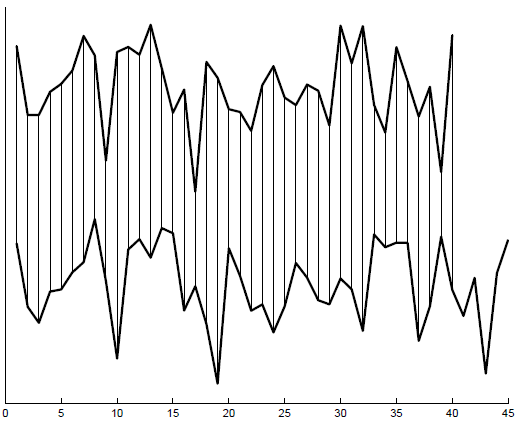
\includegraphics[width=0.5\textwidth]{./figures/euclidean_distance_time_series}
        }
        \subfloat[]{
           \label{fig:dtw_distance_time_series}
           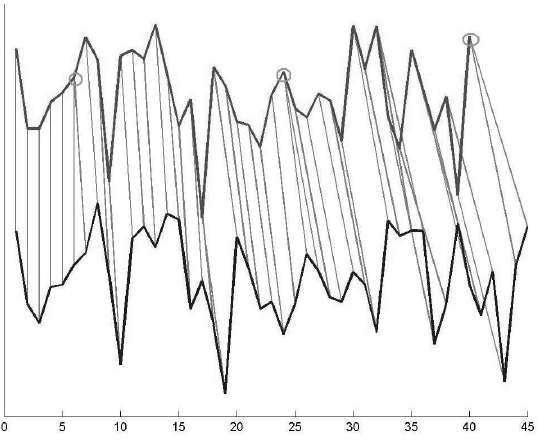
\includegraphics[width=0.5\textwidth]{./figures/dtw_distance_time_series}
        }        
    \caption{The distance between two relatively similar time series. Using the Euclidean distance as demonstrated in (a), the distance is $Minkowski_{2}(R,S)=8.68$. Using Data Time Warping as seen in (b), the distance is $DTW(R,S)=2.48$.}
   \label{fig:time_series_distance_demo}
\end{figure}

\iftoggle{edit-mode}{\hspace{0pt}\marginpar{Next Subsections}}{}
In the following two subsections (\ref{subsec:emd} and \ref{subsec:dtw}) we will explain in details two similarity measure functions used in the thesis, the \emph{Earth mover's distance} and the \emph{Data time Warping}. 

\subsection{The Earth Mover's Distance}
\label{subsec:emd}

\iftoggle{edit-mode}{\hspace{0pt}\marginpar{Introduction to EMD}}{}
The \emph{Earth Mover's Distance} (EMD), introduced by Rubner et al. in \cite{rubner2000earth}, is a measure of the dissimilarity between histograms. It was experimentally verified to capture well the perceptual notion of a difference between images. It is commonly used in content-based image retrieval to compute distances between the color histograms of two digital images \cite{grauman2004fast}.\\

\iftoggle{edit-mode}{\hspace{0pt}\marginpar{Binwise based measures}}{}
Histogram based descriptors, such as SC, are in many cases compared using a bin-wise dissimilarity techniques such as the Minkowski distance (as defined in Equation \ref{eq:minkowski}) or the $\chi^2$ statistic as defined below.\\
 
\begin{definition}
Given two histograms $H=\{h_i\}_{i=1}^{\ell}$ and $K=\{k_i\}_{i=1}^{\ell}$ the following is defined as the $\chi^2$ statistic: 
\begin{equation}
dist_{\chi^2}(H,K)=\sum_{i}^{\ell} \frac{(h_i - m_i)^2}{m_i}
\end{equation}
where $m_i=\frac{h_i+k_i}{2}$.
\end{definition}

\iftoggle{edit-mode}{\hspace{0pt}\marginpar{Drawback of binwise based measures}}{}
Bin-wise dissimilarity measures can be computed very fast due to the fact that they measure dissimilarities between the content of corresponding bins of the two histograms and discard information across bins. However, they usually fail to consider local and global variations. These variations, which would be perceived as minor by a human, may result in a large dissimilarity values between two histograms.\\

\iftoggle{edit-mode}{\hspace{0pt}\marginpar{The transportation problem}}{}
Generally speaking, the distance between two histograms can be viewed as a special case of the well-known \emph{transportation problem}, a.k.a the Monge-Kantorovich problem \cite{rachev1985monge} defined below (Definition \ref{def:transportation_problem}). Accordingly, EMD is based on the solution to the transportation problem, for which efficient algorithms are available. \\

\begin{definition}
\label{def:transportation_problem}
Given several \emph{suppliers} and \emph{consumers}. Each supplier, $P_i$, having a given amount of goods $p_i$, and each consumer, $Q_j$, having a given amount of demand, $q_j$. For each supplier-consumer pair, the cost of transporting a single unit of goods is $d_{ij}$. The transportation problem is then to find the a least expensive flow of goods from supplier to consumer that satisfies the consumer's demand, i.e., finding the flow $f_{ij}$ between $P_i$ and $Q_j$ which minimizes:
\begin{equation}
COST(P,Q,F)=\sum_{i,j} d_{ij}f_{ij} 
\end{equation}
subject to the following constrains:
\begin{equation}
f_{ij} \geq 0, 1\leq i \leq m \wedge 1\leq j \leq n 
\end{equation}
\begin{equation}
\sum\limits_{j=1}^{n} f_{ij} \leq p_i, \forall 1\leq i \leq m
\end{equation}
\begin{equation}
\sum\limits_{i=1}^{m} f_{ij} \leq q_j, \forall 1\leq j \leq n
\end{equation}
\begin{equation}
\sum\limits_{i,j} f_{ij} = \min\left\{ \sum\limits_{j=1}^{n} q_j, \sum\limits_{i=1}^{m} p_i \right\}
\end{equation}
\end{definition}

\iftoggle{edit-mode}{\hspace{0pt}\marginpar{EMD definition}}{}
Once the general transportation problem is solved, and optimal flow $f$ was found, EMD is defined as the cost normalized by the total flow, namely the total weight of the smaller histogram. which is done in order to avoid favoring small histograms. i.e.:
\begin{equation}
EMD(P,Q)=\min\limits_{f} {\frac{\sum_{i,j} f_{ij}d_{ij}}{\sum_{i,j} f_{ij}}}
\end{equation} 

EMD is a natural and intuitive metric. Descriptively, if the histograms are interpreted as two different ways of piling up a certain amount of sand, the EMD is the minimal cost of turning one pile to other. Namely, the minimal total ground distance traveled, weighted by the amount of sand moved (called flow). When used to compare histograms with the same overall mass, namely distributions, EMD is a metric.\\

\iftoggle{edit-mode}{\hspace{0pt}\marginpar{EMD modeling as flow in graph}}{}
EMD can also be modeled as a network flow problem in graph theory. The two compared histograms are represented by a bipartite graph in which each bin is represented as a vertex and its content as the vertex value. An edge connects each bin in the left graph to every bin in the left graph. The edge's weight equals to the ground distance between the two bins. The vertices in the left side graph act as sources and the vertices in the right side as sinks. Computing EMD is now the \emph{uncapacitated minimum cost flow} problem and can be solved using Orlin's algorithm in $O(N^3 logN)$ for N-bins histograms \cite{shirdhonkar2008approximate}.\\

\iftoggle{edit-mode}{\hspace{0pt}\marginpar{EMD in Feature space}}{}
As seen in previous sections, both CS and MAD produce histograms. The implementation used in this work for the SC produces a feature vector with a constant total mass, i.e., a distribution. In this case, EMD is a true metric, therefore, properly fit our needs.\\

\iftoggle{edit-mode}{\hspace{0pt}\marginpar{EMD in handwriting recognition}}{}
EMD was used by Saabne in \cite{saabni2013efficient} to measure similarity between shapes for recognizing and searching Arabic words. However, for the best of our knowledge, this is the first use of EMD for on-line handwriting recognition.\\

\iftoggle{edit-mode}{\hspace{0pt}\marginpar{EMD drawback}}{}
The major hurdle to using EMD is its $O\left( {{N^3}\log N} \right)$ computational complexity (for an $N$-bin histogram). The complexity is magnified when the task is to search for similar shapes (nearest neighbors) in a large database. In this case, a linear scan of the database would require computing a comparison of superpolynomial complexity for each database member against the query shape \cite{grauman2004fast}. In Section \ref{subsec:approximating_emd_using_embedding}, we will discuss an EMD embedding technique which greatly reduces the computation effort in approximating the EMD distance between two objects and also facilitates the application of indexing which spares the linear scan of the entire database.\\

\subsection{Data Time Warping}
\label{subsec:dtw}

\iftoggle{edit-mode}{\hspace{0pt}\marginpar{Introduction}}{}
\emph{Dynamic time warping} (DTW) is an algorithm for finding the optimal alignment between two time series. Intuitively, the sequences are warped in a non-linear fashion to match each other. See Figure \ref{fig:dtw_dequence_demo}. It was developed originally for speech recognition\\ 


DTW is used for solving the discrepancy between intuition and calculated distance using the alignment between the two sequences. It is done by accumulating the distance of the alignment path, i.e., summing the distance between every two corresponding points on the warping path. 

\begin{figure}[h!] 
\centering
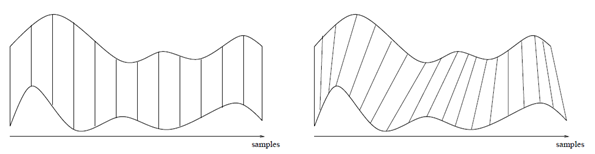
\includegraphics[width=1\textwidth]{./figures/dtw_dequence_demo}      
\caption{The right scheme shows sample-by-sample na\"{\i}ve alignment after re-sampling and in the left scheme the alignment was performed using DTW }
\label{fig:dtw_dequence_demo}
\end{figure}

\iftoggle{edit-mode}{\hspace{0pt}\marginpar{Warping path Definition}}{}
\begin{definition}
Given two time series, $X = (x_1,x_2,...,x_n)$ and $Y = (y_1,y_2,...,y_m)$, the \emph{warping path} $W=(w_1,w_2,...,w_K)$ where ${w_k} = (i_k,j_k)$ is an alignment between the two sequences which satisfies the following conditions: 
\begin{enumerate}
\item Start and End point constraint: $w_1 = (1,1)$ and $w_k = (n,m)$. 
\item Local continuity constraint: ${w_{k + 1}} - {w_k} \in \left\{ {\left( {1,1} \right),\left( {1,0} \right),\left( {0,1} \right)} \right\}$
\end{enumerate}	 
The weight of a given warping path $W$ is defined as:
\begin{equation}
G(W) = \sum\limits_{k = 1}^{K} d(x_{i_k},y_{j_k} )
\end{equation}
where $d(x_{i_k},y_{j_k})$ is the distance between the points $x_{i_k}$ and $y_{j_k}$.
\end{definition}

\iftoggle{edit-mode}{\hspace{0pt}\marginpar{DTW Definition}}{}
Equipped with the definition of a warping path, DTW is defined as follows:
\begin{equation}
DTW(X,Y)=\min\limits_{W} {G(W)}
\end{equation}
Namely, DTW returns the the weight of the path which is associated with the optimal alignment.\\

\iftoggle{edit-mode}{\hspace{0pt}\marginpar{Accumulated distance matrix}}{}
Using a dynamic programing approach, DTW yields the optimal warping path by constructing the \emph{accumulated distance matrix} $D \in \mathbb{R}^{m \times n}$. 
$D(i,j)$ is the minimum distance warping path that can be constructed from the two time series $X = \left( {{x_1},{x_2},...,{x_i}} \right)$ and $Y = \left( {{y_1},{y_2},...,{y_j}} \right)$. \\

The accumulated distance matrix is calculated as follows: 
\begin{algorithm}
$D(1,1) = 0$\;
\For{$i\leftarrow 2$ \KwTo $n$}{
	$D(i,1) = d(x_i,y_1)$\;
}
\For{$i\leftarrow 2$ \KwTo $m$}{
	$D(1,j) = d(x_1,y_j)$\;
}
\For{$i\leftarrow 2$ \KwTo $n$}{
	\For{$j\leftarrow 2$ \KwTo $m$}{
		$D(i,j) = d(x_i,y_j) + \min {\left\{D(i,j - 1),D(i - 1,j),D(i - 1,j - 1)\right\}}$\;
	}
}
\caption{Accumulated distance matrix ($D$) construction}
\label{alg:adm_dtw}
\end{algorithm}


Therefore, the value in $D(m,n)$ contains the minimum-distance warping path between $X$ and $Y$.
The optimal warping path $W$ is retrieved by backtracking the matrix $D$ from the point $D(m,n)$ to the point $D(1,1)$ following the greedy strategy of looking for the direction from which the current distance is taken \cite{senin2008dynamic}.\\

\iftoggle{edit-mode}{\hspace{0pt}\marginpar{stroke trajectories similarity measure using DTW}}{}
Handwritten strokes can be seen as temporal sequences in the planar space. In the on-line handwriting recognition, the exact temporal information is discarded in most cases by resampling the strokes to obtain equidistant sampling. However, unlike off-line handwriting recognition, the ordering information of the samples is kept. As such, DTW is an intuitive method for calculating the correspondence between two strokes. 
It have been proved relatively efficient and effective for shape matching of handwritten words. DTW was used in \cite{rath2003word, rath2003indexing, moghaddam2009application} to calculate the similarity between handwritten script in historical documents. Saabne has used DTW for key-word searching in \cite{saabni2011fast, saabni2008keyword}. \\

\iftoggle{edit-mode}{\hspace{0pt}\marginpar{DTW Speedup}}{}
One drawback of DTW is its quadratic time and space complexity, i.e., $O(mn)$ where $m$ and $n$ are the time series lengths. Therefore, several speedup methods have evolved. These methods fall into the following categories:
\begin{enumerate}
\item Constraints Enforcing: Limiting the amount of calculated cells in the accumulated distance matrix.
\item Data Abstraction: Running the DTW algorithm on an abstract representation of the data.
\item Pruning: Reducing the times DTW needs to run when determining similarity of time series.
\end{enumerate}

\paragraph{Constraints Enforcing:} 
In some cases DTW tends to create an unrealistic correspondence between time-series features by aligning short features from one of the series to the long features on the second time series. To avoid this undesired phenomenon, constrains can be imposed on the possible correspondence between several consecutive points on the warping path. Two such constraints are the Sakoe-Chuba Band \cite{sakoe1978dynamic} and he Itakura parallelogram \cite{itakura1975minimum} (Figure \ref{fig:dtw_dequence_demo}). The grayed out area is the cells of the $D$ matrix that are filled by the DTW algorithm for each constraint. The warping path is looked for in the constraint window. The width of the window is specified by a parameter. Note that such constrains limit the amount of calculation needed for computing DTW, however, the speedup factor is a constant and the DTW complexity remains quadratic. Furthermore, if the warping path is does not reside in the constraint window, it will not be found by DTW, thus, such method is usually used when the warping path is expected to be in the constrain window.

\begin{figure}
\centering
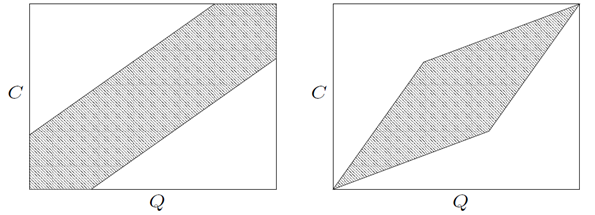
\includegraphics[width=0.7\textwidth]{./figures/dtw_sukoe_chuba}       
\caption{Cost matrix constraints: Sukoe-Chuba Band (left) and the Itakura Parallelogram (right).}
\label{fig:dtw_sukoe_chuba}
\end{figure}

\paragraph{Data Abstraction:} Speedup using data abstraction is performed by running DTW on a reduced presentation of the data thus reducing the cell numbers that need to be computed. The warp path is calculated on the reduced resolution matrix and mapped back to the original (full) cost matrix. \emph{FastDTW} which was proposed in \cite{salvador2007toward} is an example of such approach. 
 
\paragraph{Pruning:} Searching the most similar time series in the database given a template time series can be done more efficiently using lower bound functions than using DTW to compare the template to every series in the database. A lower-bounding is cheap and approximate. However, it underestimates the actual cost determined by DTW. It is used to avoid comparing series by DTW when the lower-bounding estimate indicates that the time series is worse match than the current best match \cite{rath2003word} (lower bounding benefits will be discussed in more details in Section \ref{subsec:lower_bounding_indexing}).\\

\iftoggle{edit-mode}{\hspace{0pt}\marginpar{How DTW is used in this work?}}{}
In this work, DTW is used for candidates scoring (described in chapter \ref{sec:candidates_scoring}) rather than similar samples spotting. Actually, nearest neighbors are found among the entire dataset based on the EMD metric. Next, DTW is employed for measuring the similarity between the test sample and its nearest neighbors


%%%%%%%%%%%%%%%%%%%%%%%%%%%%%%%%%%%%%%%%%%%%%%%%%%%%%%%
\newpage{}
%%%%%%%%%%%%%%%%%%%%%%%%%%%%%%%%%%%%%%%%%%%%%%%%%%%%%%%

\section{Similarity Search}
\label{sec:similarity_search}
 
\iftoggle{edit-mode}{\hspace{0pt}\marginpar{Introduction}}{}
In Section (\ref{sec:similarity_measures}) we have discussed the first aspect of information retrieval - the effectiveness of measuring the perceptual notion of similarity between two objects. However, even the most qualitatively effective similarity technique is almost useless, if the task searching for similar objects, for a given query object, in the database cannot be done efficiently. In this chapter, we will discuss this aspect of information retrieval, namely how to build a data-structure methods for fast retrieval of the conceptually nearest object to a given query object. Keeping the similarity search efficient as much as possible requires the development of search methods that minimizes the overall search costs.\\

\iftoggle{edit-mode}{\hspace{0pt}\marginpar{Similarity search query types}}{}
Similarity based search introduce two fundamental query types: \emph{range queries} and \emph{k-nearest neighbor queries} \cite{hetland2009basic}. Under the definition of a distance function given in \ref{def:distance_function}, formal definitions of both query types are provided below. See Figure \ref{fig:similarity_query_types} for a visual demonstration of the two types of queries.
\begin{definition}
Given a data space $D$, a distance function $dist$ defined on $D$, a query object $q$ and a range parameter $r \geq 0$. \textbf{Range query} returns all the data objects in $D$ that are within a distance $r$ from the query object $q$.
\begin{equation}
Range(q,r,D,dist)=\{o \in D | dist(q,o) \leq r \}
\end{equation}
\label{def:range_query} 
\end{definition}

\begin{definition}
Given a data space $D$, a distance function $dist$ defined on $D$, a query object $q$ and a range parameter $r \geq 0$. \textbf{kNN query} returns the $k$-closest objects in $D$ to the query object $q$.
\begin{equation}
k-NN(q,D,dist)=\{A \subseteq D | \forall a \in A, b \in D \setminus A: dist(q,a) \leq dist(q,b) \wedge |A|=k \}
\end{equation}
\label{def:knn_query} 
\end{definition}

\begin{figure}[h!]
	\centering
        \subfloat[]{
            \label{fig:range_query}
            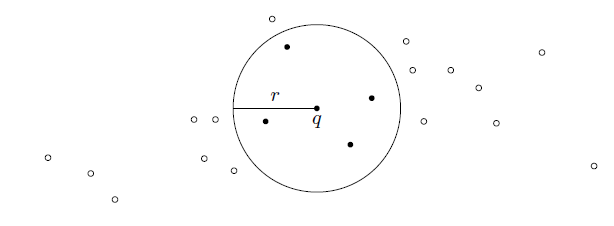
\includegraphics[width=0.5\textwidth]{./figures/range_query}
        }
        \subfloat[]{
           \label{fig:knn_query}
           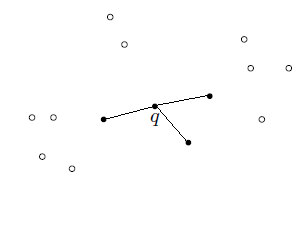
\includegraphics[width=0.5\textwidth]{./figures/knn_query}
        }        
    \caption{Visualization of a range and k-nn queries in two-dimensional Euclidean space.}
   \label{fig:similarity_query_types}
\end{figure}

\iftoggle{edit-mode}{\hspace{0pt}\marginpar{The kNN queries}}{}
While range queries are argued to be fundamental, kNN queries notably take a large volume in the literature. In the following I focus on one of the basic kinds, k-NN queries.\\

\iftoggle{edit-mode}{\hspace{0pt}\marginpar{The problem}}{}
The similarity search costs can be objectively defined as the computer time needed to evaluate a query. In the case of similarity based search, the method should minimize two components. The computation cost and the disk access cost. The computation costs represent the number of distance computations needed for a query evaluation. As discussed in Section \ref{sec:similarity_measures}, effective similarity measure methods that reasonably correspond to the human intuition are computational costly. The I/O costs are related to the volume of data needed to be transfered from a secondary memory during a query evaluation. Namely, the number of samples in the dataset to be evaluated against the query object in order to obtain the nearest samples \cite{saabni2013efficient}.\\


%\iftoggle{edit-mode}{\hspace{0pt}\marginpar{The different aspects of the problem}}{}
%It is clear that the magnitude of the dataset depends on the type of data it holds, for example, a dataset containing a letters samples is much smaller than a database that contains word part samples and thus the motivation for techniques that avoid scan of the entire database increase. For Example, searching for similar word shapes for a given query word in the English lexicon using DTW may take more than few hours on an average personal computer \cite{saabni2013efficient}. However, even for a letters based recognition, a comprehensive letters recognition database will probably have hundreds or even thousands of samples. \\

\iftoggle{edit-mode}{\hspace{0pt}\marginpar{Solution directions}}{}
in order to minimize the time needed tie for searching a similar object in a large dataset, one needs to make as few as possible distance calculations to candidates. The problem is this option is not feasible with non-metric distance functions, such as many existing similarity functions, including DTW, EMD and others. However, reducing the computation cost can be achieved by using a cheap similarity measure function to approximate (lower bound) the quantity of similarity between given two sample shapes, and filtering out candidates that their approximated similarity is larger than a preset threshold. This is type of technique is called \emph{Lower Bounding}. reducing the disc access cost can be achieved by discarding entire portion of the dataset which are assured that are distant enough (i.e., their similarity is assured to be relatively large) from the the given query object. Such techniques are called \emph{Metric Indexing} and usually require the metric to maintain several conditions.\\

\subsection{Lower Bounding}
\label{subsec:lower_bounding}

\iftoggle{edit-mode}{\hspace{0pt}\marginpar{Distance function approximation}}{}
In order to improve upon the evaluation of the distance function on every object in the dataset, we must somehow infer that an object x can be included in, or excluded from, the search result without calculating $d(q, x)$. The way to go is to find a cheap way of approximating the distance. In order to avoid wrongfully including or excluding objects, we need an approximation with certain properties. The approximated distance must either overestimate or underestimate the actual distance, and must do so consistently. For example, if the distance function $\check d$ consistently yields lower values than the actual distance function $d$ (over the same set of objects). Assuming that $\check d$ needs less effort to be calculated, a considerable speedup will be obtained by using the following algorithm for finding the nearest neighbor for a given query object $q$ \cite{keogh2005exact}.\\

\begin{algorithm}
$best\_so\_far = \infty$\;
\For{every sequence $x$ in database}{
	\If{$\check{d}(q,x) < best\_so\_far$}{
		$dist = d(q,x)$\;
	}
	\If{$dist < best\_so\_far$}{
		$best\_so\_far = dist$\;
		$nearest\_neighbor = x$\;
	}
}
\caption{An algorithm that uses a lower bounding distance measure to speed up the sequential scan search for the query q}
\label{alg:lower_bound}
\end{algorithm}

\iftoggle{edit-mode}{\hspace{0pt}\marginpar{Lower Bounding advantage}}{}
Although, both lower and upper bounding measures can be exploited to avoid running the expensive $d$ calculation, lower bounding appears to be more useful as it can be safely used to exclude far candidates as described in Algorithm \ref{alg:lower_bound}. The more the approximation is accurate the less the actual distance function $d$ will be invoked. However, there will normally be a tradeoff between approximation quality and cost of computation. 

\subsection{Metric Embedding}
\label{subsec:metric_embedding}

The speed up achieved by lower bounding is usually small (about 10 times faster). A different approach for solving the number of the distance function calculation is by embedding the feature vectors into a metric space equipped with a simple-to-compute metric function  so that the calculation of distances between two feature vectors will be approximated inexpensively. And using the triangular equality of the metric space sub-linear scan of the dataset can be obtained.\\

\begin{definition}
Given metric spaces $(X, d)$ and $(X', d')$ a map $f : X \rightarrow X'$ is called an embedding. An embedding is called distance-preserving or isometric if for all $x, y \in X$, $d(x, y) = d'(f(x), f(y))$.
\end{definition}

\iftoggle{edit-mode}{\hspace{0pt}\marginpar{Distortion}}{}
It is very rare to find cases where isometric embeddings can be found between two spaces of interest, and hence we often have to allow the mappings to alter distances in some (hopefully restricted) fashion. The reason we do embedding is to be able to more cheaply calculate the distance function. Usually, the embedding will be into a space in which the distance function is cheap and the distance in the embedded approximate the distance of the distance space. There are many notions of "close"; most of the course will focus on the following notions.

\begin{definition}
Given two metrics $(X, d)$ and $(X',d')$ and a map $f : X \rightarrow X'$, the contraction of $f$ is the maximum factor by which distances are shrunk, i.e.,
\begin{equation}
\max_{x,y \in X} \frac{d(x,y)}{d'(f(x),f(y))}
\end{equation}

The expansion or stretch of f is the maximum factor by which distances are stretched:
\begin{equation}
\max_{x,y \in X} \frac{d'(f(x),f(y))}{d(x,y)}
\end{equation}
and the distortion of $f$, denoted by $\|f\|_{dist}$, is the product of the distortion and the expansion.
\end{definition}

%Another equivalent definition is the following: the distortion of $f$, is the smallest value $\alpha \geq 1$ for which there exists an $r > 0$ such that for all $x, y \in X$
%\begin{equation}
%rd(x, y) \leq d'(f(x), f(y)) \leq \alpha r d(x, y)
%\end{equation}

\subsection{Approximating EMD using Embedding}
\label{subsec:approximating_emd_using_embedding}

\iftoggle{edit-mode}{\hspace{0pt}\marginpar{$L_p-norm$ advantage and drawbacks}}{}
Using normed spaces such as $L_p-norm$ (see Definitions \ref{def:norm} and \ref{lp_norm}) to solve the dissimilarity measure problem enables using data structures which are specifically designed for points living in the normed space, such as k-d trees and R-trees. 
Such data structures provide mechanisms for answering the kNN query in an orders of magnitude faster than linear scan of the database. However, the quality of the dissimilarity measure of such norms, as mentioned before, is not always satisfactory \cite{indyk2003fast}.\\

\begin{definition}
Given a data space $D$, for any two data elements  $x,y \in D$, a \textbf{norm} $\|\cdot\|$ is defined as:
\begin{equation}
\|\cdot\|: D \longrightarrow \mathbb{R}
\end{equation}
where the following conditions hold:
\begin{itemize}
\item $\|x\|=0 \Leftrightarrow x=0$
\item $\|x-y\| \geq|\|x\|-\|y\||$
\item $\|\alpha x\|=|\alpha|\|x\|$
\end{itemize}
the pair $\left(D,\|\cdot\|\right)$ is called a \textbf{normed space}.
\label{def:norm}
\end{definition}


\begin{definition}
Given an vector space $V=\mathbb{R}^N$ and $v=(v_1,v_2,...,v_N) \in V$, $L_p-norm$ is defined as:
\begin{equation}
\|v\|_p=\sqrt[p]{\sum\limits_{i=1}^N v_i^p}
\end{equation}
\label{lp_norm}
\end{definition}

$L_p-norm$ is based on the Minkowski distance function.\\

\iftoggle{edit-mode}{\hspace{0pt}\marginpar{EMD embedding by Indyk and Thaper}}{}
Several approximation algorithms have been proposed to speed up the computation of EMD. Indyk and Thaper, in \cite{indyk2003fast}, has suggested a technique in which the un-normed EMD metric is embedded into a normed space $L_1$ norm, so that the distance between the two objects, in their case images, is comparable to the distance between the two points which represent the embedding of the two images. We will refer to this embedding as $L_1-EMD$. The Embedding time complexity is $O(Nd log{\Delta}$, where $N$ is the feature set size, $d$ is the feature space dimension and $\Delta$ is the diameter of the union if the two feature sets.\\

%Working in a normed space is desirable since fast approximate NN search techniques such as LSH require it. ????

%\iftoggle{edit-mode}{\hspace{0pt}\marginpar{Indyk $L_1-EMD$ embedding details}}{}
\subsubsection{EMD Embedding into $L_1$}
As described in Section \ref{}, EMD can be viewed as a generalization of the distance between points to distance between sets of points. 
For a given two points sets $A$ and $B$, both of cardinality $n$ and containing points in $L_2^d-metric$ and $C=A \bigcup B$, the embedding proposed in \cite{indyk2003fast} is into the $L_1^d-norm$ (i.e. the space of vectors in $\mathbb{R}$ equipped with the Manhattan norm). 
The general idea of the embedding is to compute and concatenate several weighted histograms of decreasing resolution for a given point set as follows: 
Let us assume that the smallest distance between any two points is $1$ and $\Delta$ is the diameter of $C$, the embedding can be described as imposing hierarchy of grids $G_i$ having side length $2^i$ on the space $\mathbb{R}^d$, where $-1 \leq i \leq log(\Delta)$. It is required that each grid $G_{i}$ is a refinement of the grid $G_{i+1}$. 
Each grid is translated by a vector chosen randomly from $[0, \Delta]^d$. Then for each grid $G_i$ create a vector $v_i(A)$ with one coordinate per cell which contains the number of points in the corresponding cell, i.e. $v_i(A)$ forms a histogram of A. The embedding, denoted as $f(A)$, is then defined as the concatenated vector of the $v_i$'s, scaled by the grid side lengths:
\begin{equation}
f_{EMD}(A) = [v_{-1}(A)/2, v_0(A), 2v_1(A), 4v_2(A),..., 2^iv_i(A),...]
\end{equation} 
An image visually describing the embedding is given in Figure {}.\\

Approximating the EMD distance between the set $A$ and $B$ is then done by calculating the Manhattan distance between the two corresponding embedding vectors, i.e.,
\begin{equation}
EMD_{approx.}=|f_{EMD}(A) - f_{EMD}(A)|
\end{equation}  

\iftoggle{edit-mode}{\hspace{0pt}\marginpar{Theoretical distortion}}{} 
The distortion of the embedding has an upper bound of $O(log \Delta))$. A detailed proof is given in \cite{indyk2003fast}. However, the proved theoretical distortion can only provide a week practical instrument. Experimental check performed on a dataset of $20,000$ objects proved a $(1+\epsilon)-approximate$ nearest neighbor, with $\epsilon < 20\%$ achieved by the embedding compared to the exact EMD. \\

\iftoggle{edit-mode}{\hspace{0pt}\marginpar{Contour matching}}{}
Based on the $L_1-EMD$ embedding proposed by Indyk and Thaper, Grauman and Darrel in \cite{} used it as a metric for contour matching, and proved the quality of retrieval from the exact versus the approximate method is less than $10\%$. They have evaluated the drop in the accuracy of the nearest neighbor retrieval from the exact EMD, to $L_1-EMD$ embedding.\\


\subsubsection{EMD Embedding into the Wavelet Coefficients Domain}
%How it is done?
%Is it faster to calculate?
%Is the retrieval more accurate (empirically) than the $L_1-EMD$ embedding?
%Are the bounds are more strict?

Note that in the original work on EMD as a metric for image retrieval in \cite{rubner2000earth}, the authors provided more general definition of EMD which does not assume $|A|=|B|$. However, in \cite{indyk2003fast} this generalization was not considered, since in this case EMD does not form a metric. Also, the shows that $EMD_{approx.}$ is equivalent to EMD averaged over all random shifts. They do not prove this for individual embedding. In this work we use an embedding technique proposed in a later work \cite{shirdhonkar2008approximate} done by Shirdhonkar and Jacobs. In their work, they has proposed a method for approximating the EMD between two low dimensional histograms using the weighted wavelet coefficients of the difference histogram. The approximation is done by transforming the histograms into $L_1$ space so that the distance between the two vectors in the wavelet domain is the EMD approximation. They have proven the ratio of EMD to wavelet EMD is bounded by constants.\\ 

\textbf{Wavelets}: the topic of wavelet and the wavelet transform is a relatively new concept (about 10 years old) which usually requires a large investment of time and a high level of mathematical background, which is not covered in a basic calculus course to be deeply comprehended.
Wavelet transform, like the Fourier transform, is used in many fields of mathematics, physics and engineering. Quite a few articles and books were written on the subject, therefore, here we will try to provide an intuitive introduction to the topic and let the interested reader to learn more about the subject in the literature.  

Recall that the Fourier Transform gives the frequency information of the signal, which means that it tells us how much of each frequency exists in the signal, but it does not tell us when in time these frequency components exist. This information is not required when the signal is so-called stationary, i.e. signals whose frequency content do not change in time. FT can be used for non-stationary signals, if we are only interested in what frequency components exist in the signal, but not interested where these occur. However, if this information is needed, i.e., if we want to know, what frequency component occur at what time (interval), then Fourier transform is not the right transform to use. Wavelet transform is capable of providing the time and frequency information simultaneously, hence giving a time-frequency representation of the signal.

Wavelets may be seen as small waves $\psi(t)$, which oscillate few times, but unlike the harmonic waves ($sin(nx)$ and $cos(nx)$ on $(-\pi,\pi]$) must die out to zero as $t \rightarrow \pm\infty$. The most applicable wavelets are those that die out after a few oscillations on a finite interval $[a,b)$. 

The wavelet transform aims to convert a signal into a series of wavelets and by doing so to provide a way for analyzing waveforms bounded in both frequency and duration. This is done to provide information that is not obvious in the original time domain function and also to allow signals to be stored efficiently and to be able to better approximate real-world signals. 

\begin{equation}
\Psi^{\psi}_{x}(\tau, s)=\frac{1}{\sqrt{|s|}}\int{x(t)\psi^*(\frac{t-\tau}{s})dt}
\end{equation}
As seen in the above equation , the transformed signal is a function of two variables, $\tau$ and $s$ , the translation and scale parameters, respectively. $\psi(t)$ is the transforming function, and it is called the mother wavelet .

The scale parameter in the wavelet analysis is similar to the scale used in maps. As in the case of maps, high scales correspond to a non-detailed global view (of the signal), and low scales correspond to a detailed view. Similarly, in terms of frequency, low frequencies (high scales) correspond to a global information of a signal (that usually spans the entire signal), whereas high frequencies (low scales) correspond to a detailed information of a hidden pattern in the signal (that usually lasts a relatively short time).
The idea of the wavelet transform is analysis a signal function $f(x)$ by creating a mathematical structures that vary is scale. i.e., construct a function, shift it by some amount, change its scale. Repeat the procedure to obtain a new approximation. This is usually refereed to as a \emph{multiresolution analysis}. In order to analyze a non-stationary signal, we need to determine its behavior at any individual event. Multi-resolution analysis provides one means to do this. A multi-resolution analysis decomposes a signal into a smoothed version of the original signal and a set of detail information at different scales. Once we have decomposed a signal this way, we may analyze the behavior of the detail information across the different scales.
The fundamental idea of wavelet transforms is that the transformation should allow only changes in time extension, but not shape. This is effected by choosing suitable basis functions that allow for this.
A function $f$ in $\mathbb{R}$ can be expressed in terms of wavelet series as:
\begin{equation}
f(x)=\sum\limits_{k}{f_k \phi(x-k)}+\sum\limits_{k}{f_{j,k}\psi_{j,k}(x)}
\end{equation}

where $\phi$ is the scaling function and $\psi$ is the wavelet. $k$ runs through all integer and represents shifts.

Converting the histograms into the wavelet domain is done by converting and its coefficients are scaled according to equation \ref{eq:emd_scaling}.
\begin{equation}
d(p)_{wemd}=\sum\limits_{\lambda}|p_{\lambda}|2^{-j(s+n/2)}
\label{eq:emd_scaling}
\end{equation}
where $p_{\lambda}$ is the wavelet transform coefficients of the difference density $p$ generated by the orthonormal wavelet-scaling function. The index $\lambda$ includes shifts and the scale j.

Computing the EMD distance in the next step is done as the $l_1$ (Manhattan) distance between these coefficients. In order to choose the wavelet domain for embedding, the authors have tested few, and showed that the Coif-lets of order 3 and the Symmetric Daubechies wavelets of order 5 had low error rates. We follow their results and use order 3 Coif-lets in
our system.

They have provided both theoretical and experimental bounds. The theoretical approximation is based on the following theorem:

\begin{theorem}
Consider the KR problem with the cost function $c(x,y)=\|x-y\|^s$, $s<1$. Let $p_k$ and $p_{\lambda}$ be the wavelet transform coefficients (approximation and details) of he difference density $p$ generated by the orthonormal wavelet scaling function pair $\psi$ and $\phi$ with regularity $r \geq q > s$. Then for any non-negative constants $C_0$ and $C_1>0$,
\begin{equation}
\hat{\mu}=C_0 \sum\limits_k{\|p_{\lambda}\|}+C_1\sum\limits_k{2^{-j(s+n/2)}\|p_{\lambda}\|}
\end{equation}
is an equivalent metric to KR metric $\dot{mu_c}$; i.e. there exist positive constant $C_L$ and $C_U$ (depending only on the wavelet used) such that
\begin{equation}
C_L\hat{\mu} \leq \dot{\mu_c} \leq C_U\hat{\mu_c}
\end{equation} 
\end{theorem} 

And the empirical bound is based on an experiment done \emph{TODO: write the test setup} they show that this metric follows EMD closely and can be used instead without any significant performance difference. The wavelet EMD metric can be computed in $O\left( N \right)$ time complexity.

Empirically the normalized RMS error obtained was between 13\% and 20\% while the embedding proposed by Indyk and Thaper achieved 43\%. In addition, the wavelet embedding surpassed the Indyk and Thaper embedding in time performance.
Note that the embedding process requires histograms, thus the vectors in the feature space had to had to be normalized.

\subsection{Metric Indexing}
\label{subsec:metric_indexing}

%\underline{Mind Map}
%\begin{enumerate}
%
%\item How Expensive is the exact NN? What is the motivation to use ANN?
%\item How good is the approximation?
%\item pruning and indexing - from the thesis.
%\item k-d tree -  is it an ANN or exact data-structure? what is the approximation parameter? is it only for the Euclidean norm? norm or metric?
%\item In case of general metric space branch and bound approach is known under the name of metric trees. Particular examples include vp-tree and BK-tree.
%\item note that LSH require only a metric space.
%\item How lower bounding can be used to generally achieve fast retrieval?
%\end{enumerate}

Note that distance function approximation techniques alone cannot avoid linearly scanning the entire dataset in a search for the nearest neighbors of an object. In order to speed up queries index structures should be build over the dataset. The main goal of an index method is to enable efficient search, either asymptotically or simply in real wall-clock time. The time cost involved in building the index is amortized over the series of queries, and is usually ignored when considering search cost \cite{hetland2009basic}. 

\iftoggle{edit-mode}{\hspace{0pt}\marginpar{Metric index definition}}{}
Efficient data retrieval in a metric dataset requires building a \emph{metric index}, namely, a data-structure that boosts the query processing. Indexing technique partition the dataset into equivalent classes such that each equivalent class contains objects that are sufficiently close to each other. However, note that this does not assure that close objects will always be contained in the same equivalent class. Each class is bounded by a hypersphere covering all the objects in the class. This requires the to satisfy the triangular equality.
Consequently, at query time the metric index is efficiently searched to locate the equivalent classes which covers the areas where the closest objects may be contained in. These classes are then exhaustively checked for the relevant objects
This allows discarding classes that surely does not contain relevant objects.

Indexing techniques can be exact, guaranteeing to return the same result as sequential scanning, or approximate, returning good matches but not necessarily the best matches. Exact methods do not allow false positives or false negatives, i.e., all of the relevant objects are required to be returned in the query result. However, the approximate methods relax this strong requirement so that a small false negatives is accepted \cite{keogh2005exact}.

\iftoggle{edit-mode}{\hspace{0pt}\marginpar{Indexing by triangular equality}}{}
The idea of using triangle inequality to remove false candidates is illustrated. Given a query object $Q$ and two objects in the dataset $R$ and $S$, the following holds: $dist(Q,S) \geq dist(Q,R) - dist(R,S)$. If $dist(Q,R)$ and $dist(R,S)$ are known, dist(Q,S) is lower bounded by $dist(Q,R) - dist(R,S)$. In the case of a range query, for a given range $r$, if $dist(Q,R)-dist(S,R) > r$, the computation of $dist(Q,S)$ can be saved since $S$ surely does not belong to the answer set \cite{chen2005similarity}.
 
Many methods were proposed to solve the kNN problem that are significantly better than a brute-force computation the distances of the entire database. However, computing nearest neighbors approximately, can to achieve significantly faster with a relatively small actual errors. \emph{Approximate nearest neighbor} (ANN) techniques allows the user to specify a maximum approximation error bound, thus enabling the user to control the trade-off between accuracy and running time. It is usually done by preprocessing the data points and into a data-structure. \\

ANN methods such as k-d trees and Locality Sensitive Hashing (LSH) have successfully applied on variety of fast similarity retrieval problems. Unfortunately, the key assumption in these procedures is that objects in the dataset lie in a metric space. As mentioned in chapter \ref{}, this assumption is not valid for many similarity measure techniques. The disadvantage of the ANN is that a large portion of these techniques requires the classified objects to reside inside a normed space. k-d tree requires a more specific $L_p$ metric space to operate in. 

\emph{TODO: give a small introduction on LSH in 1 or two sentences}

The advantage of LSH is that it operates better than kdtree in a high dimensional space. However, the strength of kdtree is that it can be used as an exact NN technique. While the the worst case scenario complexity is $O(N)$, the expected complexity is $O(log N)$ 

In this work, kdtree was the best choice we could think of and which its properties was the most suitable for our need since the dimensionality of the data was not height. After reducing the dimensionality of the samples,they are used to create a kdtree data structure.

{\color{blue}To reduce the search space,we apply a series of filters in a hierarchical manner. The earlier filters perform light processing on a large number of candidates, and the later filters perform heavy processing on a small number of candidates. In the first filter, global features and delayed strokes patterns are used to reduce candidate word-part models. In the second filter, local features are used to guide a dynamic time warping (DTW) classifi- cation. The resulting k top ranked candidates are sent for shape-context based classifier, which determines the recog- nized word-part. In this work, we have modified the classic DTW to enable different costs for the different operations and control their behavior\cite{saabni2009hierarchical}}

In our framework, sub-strokes classification is done by finding a stored letter sample that is maximally similar to the shape of the sub-stroke. For a given sub-stroke, we need to find the most perceptually close object in the sample set. Since our samples space is in $L_1$ we use NN classification method.\\

We will also consider an embedding techniques that allows us to get the best of the both fast similarity measure calculation and use the advantages of the normed space. It will allow us to approximate the EMD distance between two histograms, and since the embedding is into an $L_1$ normed space, efficient object retrieval data structures can be used.\\

Indexing techniques of measure functions is not fast enough for our application which has a strict responsiveness requirements. Thus we still need to use the euclidean space and integrating sub-linear search technique to achieve the needed performance and also we can't afford performing the computations the similarity measures mentioned above even if the number of computation is sub-linear. Thus we have taken a different approach and used embedding technique to facilitate using.\\ 

%%%%%%%%%%%%%%%%%%%%%%%%%%%%%%%%%%%%%%%%%%%%%%%%%%%%%%%
\subsubsection{k-d tree}
\label{subsubsexc:kd_tree}

\iftoggle{edit-mode}{\hspace{0pt}\hspace{0pt}\marginpar{A short introduction to kdtree}}{} 
k-d tree, a special case of binary space partitioning trees, is a data structure for storing a finite set of points from a k-dimensional space. It was proposed by Bentley in \cite{bentley1975multidimensional}. It aims at solving the problem of searching kNN in a large set of multi-dimensional points by first building a data structure based on the set of reference points. Then, given a query object, it extract the kNN using this structure.

\iftoggle{edit-mode}{\hspace{0pt}\marginpar{How it works, how the data is saved and extracted}}{} 
The k-d tree is formed as follows: Every point is either branch node or is contained in a leaf node. Every point node in the tree is associated with one of the k-dimensions and can be though of an hyperplane that divides the space into two half spaces in that dimension. Points to the left of this hyperplane are represented by the left subtree of that node and points right of the hyperplane are represented by the right subtree. Since we would like the partition of the subspace to be as equal as possible, the selection of the point to function as a branch node in every level has a great impact on the balance of the tree. The selection can be done in many ways, the most common way is to find the medial point of a number of points in the subtree. The number of points in a leaf node is also customizable and is mostly affected by the cardinality of the points in the database and k. Since, in most application the k is predefined. 

\iftoggle{edit-mode}{\hspace{0pt}\marginpar{How the NN are found?}}{}
The approximation of the k-NN using k-d tree is done by initially finding the leaf node which contain the query point. although most it is mostly probable the nearest neighbors are contained in the leaf node, it does not necessarily contain the kNN of the query point. In the approximate version of the NN retrieval, the algorithm can halt here and return the NN of a the target point using exhaustive search on the node contained in the leaf node. However, the exact kNN version of k-d tree may require the algorithm to recursively explore the other child node and look for near neighbors in the all other branches that possibly contain a closer solution to the so far found points. Exact details of the algorithm can be found in \cite{bentley1975multidimensional}.
 
\iftoggle{edit-mode}{\hspace{0pt}\marginpar{Expected time complexity}}{}
The construction time of the k-d tree is O($d N log N$). We can afford this high complexity of the construction since the this process is done in a off-line manner and theoretically will be executed mostly several times. However, this tax pays off when it it comes to the enhancement we achieve in the NN search time complexity. The impractically observed average time is $O(log N)$. The worst case scenario the running time is $O(N^{d^2})$ when d is the dimensionality of the sample elements.

\iftoggle{edit-mode}{\hspace{0pt}\marginpar{Why we chose kdtree and not LSH.}}{} 
kdtree is mostly used for solving the k-NN problem and the range problem, i.e., given a range the algorithm should return all the object in the given range. We have preferred to use kdtree is over LSH. The reason is that since the dimensionality of the resulted samples after dimensionality reduction is low as seen in chapter \ref{[]} and we are able to use kdtree for retriving the exact kNN. kdtree is sensitive to the curse of dimensionality, which do not appear in our reduced data. 

\iftoggle{edit-mode}{\hspace{0pt}\marginpar{Mention the Matlab library and the parameters we used.}}{} 
In our implementation, the built-in Matlab wrapper was used for kdtree available in the statistical toolbox and introduced in Matlab R2013B \emph{[TODO: add reference]}. The implementation can be used with different parameters such as the distance measure and the cardinality of the lead node. And it do not provide the approximate version of kdtree, only the exact one. We empirically found that the following parameters are the best for our needs: $L_1$ metric, since the EMD embedding is into the $L_1$ space and the bucket size is 50. 

\iftoggle{edit-mode}{\hspace{0pt}\marginpar{Open Issues}}{}
\begin{itemize}
\item Can we use Matlab for both approximate and exact NN? If yes, what  
\end{itemize} 

%%%%%%%%%%%%%%%%%%%%%%%%%%%%%%%%%%%%%%%%%%%%%%%%%%%%%%%
\newpage{}
%%%%%%%%%%%%%%%%%%%%%%%%%%%%%%%%%%%%%%%%%%%%%%%%%%%%%%%

\section{Clustering-based Sample set Redistribution}
\label{sec:csr}

\iftoggle{edit-mode}{\hspace{0pt}\marginpar{Motivation}}{}  
On the one hand a large and verified sample set is crucial for every learning algorithm, in particular, it is important in the handwritten pattern classification because of the variety of styles between people in their handwriting. On the other hand, a large sample set can harm the performance of the NN based recognition system, and even harm the accuracy of the recognition because of outliers. 
As can be seen in section \ref{[]}, for some letters positions many samples were collected. And for other letters smaller set of samples were collected. On the one hand, we would like to maintain the underlying letters distribution since the distribution of our sample set has a high correlation to the real world letter distribution. On the other hand, as we have mentioned before, a non proportional sample size for some letters may harm our recognition process.\\

\iftoggle{edit-mode}{\hspace{0pt}\marginpar{Introduction}}{}
Cluster analysis is a common approach used in both supervised and unsupervised learning. It aims to partition a a set of objects  into groups in such a way that objects in the same group (called a cluster) are more similar (in some sense or another) to each other than to those in other groups.
Clustering has two main uses; the first is deriving a reduced representation of the full data set. the second use is deducing new insights into the structure of the data.
Since a cluster is a notion that cannot be precisely defined, thus there is no objectively correct clustering and this is the reason there are so many clustering algorithms.
There are many clustering models. By models we mean the basic concept on which the clustering is based upon. The most prominent models are the \emph{Connectivity models}. In this group we can find the hierarchical clustering. Another widely used set of models is the \emph{Centroids models} which contain such as well known k-means algorithm. Cluster analysis is used for various goals. In non-supervised learning, when the class label are not available, this technique enable the classification system to impose classes on the sample set. In the supervised learning, it can be used to impose a hierarchy on the sample set and by doing so improving the classification performance and accuracy.\\

\iftoggle{edit-mode}{\hspace{0pt}\marginpar{What type of clustering did we use, and why. $L_1$ K-medoids}}{}
The problem of disproportional number of samples per letter class we solved by using the clustering k-medoids algorithm. the k-medoids algorithm aims to break up the dataset into k clusters. A medoid is a representative object of a cluster whose average dissimilarity to all the objects in the cluster is minimal. The k-medoids algorithm finds the k medoids of a dataset. 
k-medoids can work with an arbitrary matrix of distances between data points. In our case the distance function is $L_1$. 
Our decision to use the k-medoids algorithm rather than the common k-means algorithm is derived from obtain a digest of the dataset. Thus the returned $k$ objects by the k-medoids algorithm will function as the representatives of the samples in a given class.\\

\iftoggle{edit-mode}{\hspace{0pt}\marginpar{Short description of the k-medoids algorithm}}{}
k-medoids operates as follows: first it selects $k$ objects in random, named $M$ of the in datapoints and associate each datapoint to the closest object in $M$. Then, for each element $m$ in $M$ and for each object $o$ in the data set, swap $m$ and $o$ and compute the the total cost of of the configuration, and select the configuration, with the lowest cost. Repeat the mentioned until the is no change in the set $M$. \emph{TODO: fix this flabby description.} \\ 


\iftoggle{edit-mode}{\hspace{0pt}\marginpar{When it is applied? How did we determine the number of clusters per each letter, and the number of elements in each cluster.}}{}
As mentioned before, the number of sample instances per class may greatly affect the classification result. Thus, we would like that the number of samples of each class will be distributed correspondingly to the apriory probability of the appearance of the letter in a given text. Since the letters were taken from the same database as the test set, it could have achieved optimistic results since the lexicon is the same lexicon of ~930 Tunisian cities. Thus the redistribution of letters according there apriori probability to the general Arabic text probability. We pretend to to be context free, thus this step is necessary. In addition to the fact the we have achieved very disproportion of class representative in the sample set. \\    

\iftoggle{edit-mode}{\hspace{0pt}\marginpar{How did affect our results.}}{}  
On the one hand, as claimed above, leaving the original distribution may result in a too good results since it will distributed according the the letters aproiri probability appearance. On the other hand the classification results may be hurt because of outliers that affect the NN algorithm. Here we would like to show classification results of before and after samples redistribution. In the following table we show the results of the test we have conducted as follows: We have created a test set of letters and reported the percentage of the recognition rate.\\
 
%%%%%%%%%%%%%%%%%%%%%%%%%%%%%%%%%%%%%%%%%%%%%%%%%%%%%%%
\newpage{}
%%%%%%%%%%%%%%%%%%%%%%%%%%%%%%%%%%%%%%%%%%%%%%%%%%%%%%%

\section{Dimensionality Reduction}
\label{sec:dr}

\iftoggle{edit-mode}{\hspace{0pt}\marginpar{What is DR and what techniques are there?}}{}
\emph{Dimensionality Reduction} is a process of reducing the number of variables taken into consideration in the learning and classification of data. It is a very important process in machine learning since it facilitates classification, efficient storing and visualization of high-dimensional data. The undesired properties of high-dimensional data present many mathematical challenges and practical complications \cite{van2009dimensionality}. First, Analysis of high-dimensional data generally requires a large amount of memory and computation power, which may be impractical for on-line classification systems and obstructive in other applications. In particular, many NN methods such as k-d tree are ineffective when the dimensionality of the data is high.
Second, the classification algorithm is more likely to overfit the training sample and generalizes poorly to new samples \cite{aida2009word}.\\

\iftoggle{edit-mode}{\hspace{0pt}\marginpar{data Intrinsic dimensionality}}{}
Ideally, the reduced representation should have a dimensionality that corresponds to the intrinsic dimensionality of the data \cite{van2009dimensionality}.
The intrinsic dimensionality of data is the minimum number of parameters needed to account for the observed properties of the data.\\ 

\iftoggle{edit-mode}{\hspace{0pt}\marginpar{The underlying belief}}{}
The belief underlying the existence of a compact representation of the external world data is based on the observation that the human brain can instantaneously and precisely recognize an observed apple, smile or a handwritten letter within a short route of neural computations. However, a digital representations of these images may consist of hundreds or thousands of pixels. Thus, clearly, there are much more compact representations of images, sounds, and even text than their native digital formats. Many recently proposed dimensionality reduction techniques are based on the intuition that data lies on or near a complex low-dimensional manifold that is embedded in the high-dimensional space.\\

\iftoggle{edit-mode}{\hspace{0pt}\marginpar{The curse of dimensionality}}{}
The high dimensional data phenomenon is widespread in data analysis and was given the name \emph{the curse of dimensionality}. In many pattern recognition applications, the problem of high dimensional data can arise in different stages of the learning and classification process; 1. the dimensionality of the data may be high in the first place; 2. features calculated on the data may be impractically large; 3. other manipulations performed on the data, such as the embedding used in this work, may produce highly dimensional vectors. \\

\iftoggle{edit-mode}{\hspace{0pt}\marginpar{Mathematical Definition}}{}
Mathematically, given $p$-dimensional variable $x \in \mathbb{R}^p$, the dimensionality reduction process finds a lower dimensional representation $s \in \mathbb{R}^k$ with $k \leq p$ which preserves the content of the original data under a given criterion. The reduced dimensionality $p$ is chosen to be as small as possible, but yet sufficiently large to guarantee that the output vector $s$ provide a faithful representation of the input vector $x$. Dimensionality reduction techniques can be classified into linear and non-linear. Linear dimensionality reduction is based on a linear projection of the data assuming the data resides close to a lower dimensional linear subspace. Namely, each of the components in the vector $s$ is a linear combination of the components in the vector $x$, formally:
\begin{equation}
s=Wx
\end{equation}
where $W_{k \times p}$ is the linear transformation.\\

\iftoggle{edit-mode}{\hspace{0pt}\marginpar{Linear DR}}{}
\emph{Principal component analysis} (PCA) and \emph{linear discrimination analysis} (LDA) are traditional linear dimensionality reduction techniques.\\

\iftoggle{edit-mode}{\hspace{0pt}\marginpar{Non-Linear DR}}{}
In some cases, linear dimensionality reduction techniques perform poorly and a more powerful approach is required to provide the mapping from the high dimensional space to the low dimensional space. In such cases, non-linear techniques is are used. Yet, the drawback of such technique is concealed in its generality which may cause over-fitting the sample set and not really capture the true underlying coordinate system. Commonly used non-linear technique include \emph{Kernel PCA}, \emph{Isometric Feature Mapping} (ISOMAP) and \emph{Locally-linear embedding} (LLE).\\

\iftoggle{edit-mode}{\hspace{0pt}\marginpar{Why do we need DR?}}{}
The need for employing dimensionality reduction in this work emerged from the sparse vectors produces by the EMD embedding of the feature vectors into the wavelet domain procedure which was described in section \ref{subsec:approximating_emd_using_embedding}. This process produced vectors in $R^{3946}$. The wish to employ k-d trees, which is very sensitive to high dimensional data, was the main reason for using dimensionality reduction. An alternative was to use a k-NN data-structure that performs well with high dimensional data such as LSH \cite{gionis1999similarity}. However, it would be less accurate since LSH is an approximate NN search method, unlike k-d tree which finds the exact k-NN samples.\\

\iftoggle{edit-mode}{\hspace{0pt}\marginpar{What DR we use?}}{}
In this thesis we have chosen to work only with linear dimensionality reduction techniques. PCA and LDA were applied sequentially in order to obtain linearly discriminative information in an efficient manner.\\

\iftoggle{edit-mode}{\hspace{0pt}\marginpar{PCA}}{}
\emph{Principle Component Analysis} (PCA) was invented in 1901 by Karl Pearson. Although there are many linear dimensionality reduction techniques, PCA is by far the most popular. PCA is unsupervised in the sense that the labeling of the data do not effect the determination of the transformation function. It produces an orthogonal linear transformation that transforms the data to a new coordinate system such that the greatest variance by any projection of the data comes to lie on the first coordinate (the first principal component), the second greatest variance on the second coordinate, and so on (as seen in figure \ref{fig:pca_demo}). The principal components as a whole form an orthogonal basis for the space of the projected data. Given a multivariate dataset visualized as a set of coordinates in a high-dimensional data space, PCA obtains the "shadow" of that dataset when viewed from its most informative viewpoints by projecting the dataset into a lower-dimensional space. This is done by using only the first few principal components.\\

\begin{figure}
\centering
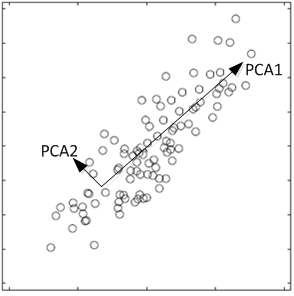
\includegraphics[width=0.5\textwidth]{./figures/pca_demo}       
\caption{The first and second principal component, PCA1 and PCA2 respectively.}
\label{fig:pca_demo}
\end{figure}

\iftoggle{edit-mode}{\hspace{0pt}\marginpar{PCA formulation}}{}
In computational terms the principal components are found by calculating the eigenvectors and eigenvalues of the data covariance matrix. This process is equivalent to finding the axis system in which the co-variance matrix is diagonal. The eigenvector with the largest eigenvalue is the direction of greatest variation, the one with the second largest eigenvalue is the (orthogonal) direction with the next highest variation and so on. The eigenvalues represent the distribution of the source data's energy among each of the eigenvectors, where the eigenvectors form a basis for the data. The representation content $g$ for the $j^{th}$ eigenvector is the sum of the energy content across all of the eigenvalues $\lambda_k$ from 1 through $j$ :
\begin{equation}
g[j]=\sum_{k=1}^{j}\lambda_k \text{   for   } j=1,...,d,
\end{equation}
where $d$ denotes the dimensionality of the original data. The \emph{data preservation rate} value (E) is calculates as seen in Equation \ref{eq:dr_energy}. 

\begin{equation}
E[L] = \frac{g[L]}{g[d]}
\label{eq:dr_energy} 
\end{equation} 

The goal is to find the smallest possible value of $L$ that achieves $E[L]$ value which rise above a preset threshold $e$, usually larger than 0.9. This approach is a well-known dimensionality estimation technique known as the \emph{eigenvalue-based dimensionality estimator}. It is a member of the \emph{global dimensionality estimator} family. Later on in this section we will mention other type of dimensionality estimator family named \emph{local dimensionality estimator}.\\

\iftoggle{edit-mode}{\hspace{0pt}\marginpar{LDA}}{}
The major drawback of PCA is that it is an unsupervised technique and as such does not use label information of the data. The following example, given by Welling in \cite{welling2005fisher}, demonstrates the problem in using PCA: in figure \ref{fig:cigarettes_data}, we see two cigar like clusters. The samples in the upper cigar are classified as $y=1$ and the samples in the other cigar are classified as $y=-1$. The cigars are parallel and very close to each other. The variance of the entire sample set, disregarding the labels, is in the direction of the cigars. Projecting the sample set on the principal component, in this case, would be terribly mix the samples. Clearly, a better projection would be orthogonal to the cigars, namely in the direction of least overall variance, which would perfectly separate the two classes.
LDA, a descendant of the original Fisher-LDA that was proposed by Fisher in \cite{fisher1936use}, overcomes this problem. Unlike PCA, LDA is a supervised technique, i.e., it explicitly attempts to model the difference between classes of data based on the samples labeling. In this method, variability among the feature vectors of the same class is minimized and the variability among the feature vectors of different classes is maximized. LDA performs dimensionality reduction while preserving as much of the class discriminatory information as possible. A brief tutorial on LDA is given in \cite{balakrishnama1998linear}. Without going into the math, in order to find a good projection vector, we need to define a measure of separation between the projections. The solution proposed by Fisher is to maximize a function that represents the difference between the means, normalized by a measure of the within-class scatter. LDA has three main drawbacks; the first is that it assumes that the data resides in $L_2$; second, LDA assumes that the distribution of the samples in each class is Gaussian which is not necessarily true for our samples; third, it is much slower to calculate compared to PCA.\\

\emph{TODO: LDA demo image.}\\

\begin{figure}
\centering
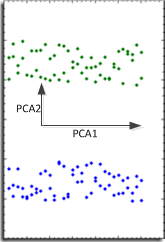
\includegraphics[width=0.3\textwidth]{./figures/cigarettes_data}       
\caption{A cigarettes like samples data spread. In this case PCA performs badly.}
\label{fig:cigarettes_data}
\end{figure}

\iftoggle{edit-mode}{\hspace{0pt}\marginpar{Why do we use both LDA and PCA?}}{}
Even though LDA is preferred in many application, it does not always outperform PCA. In order to optimize discrimination performance in a more generative way, a hybrid dimension reduction model combining PCA and LDA is used in this work.\\

\iftoggle{edit-mode}{\hspace{0pt}\marginpar{When to perform the DR?}}{}
Grauman et al. in \cite{grauman2004fast} used PCA to find a low-dimensional subspace based on a large sample of the shape context histogram. PCA yields the set of bases that define a low-dimensional "shape context manifold". Only then the approximate EMD embedding is performed. However, we have chosen to perform the stages in a different order. First, approximate EMD embedding is performed on the feature vectors, and only then, dimensionality reduction procedure is applied to reduce the dimensionality of the sparse embedded vectors. The reason we have chosen to perform the stages in this order is that if we were to apply the order suggested by Grauman, we would still result in a large sparse vectors constructed by the embedding process.\\
  
\iftoggle{edit-mode}{\hspace{0pt}\marginpar{Usage of PCA in the $L_1$ space.}}{}
The basic form of PCA is defined over the $L_2$ space. However, the data that is embedded to the wavelet domain was proved to approximate EMD in the $L_1$ space. Although $L_1$-PCA techniques were examined in the literature \cite{kwak2008principal}, we decided to use the basic form of PCA, given that $L_2$ estimate $L_1$ fairly well.\\

\iftoggle{edit-mode}{\hspace{0pt}\marginpar{Implementation: PCA}}{}
In the proposed system, we wanted to exploit the strengthens of both PCA and LDA techniques using the dimensionality reduction process which is outlined as follows: The samples are projected to a subspace $S_1$ using PCA and then to subspace $S_2$ using LDA. In the PCA stage, the target dimensionality, i.e., the number of principal components taken into consideration, is the minimal to achieve data preservation rate of 99\%, i.e., $E=0.99$. As mentioned before, the dimensionality of the original vectors was 3946. The reason we adopted such a high rate is that it was enough to achieve a very major dimensionality reduction. As seen in table \ref{table:dr_dimensions_results}, the dimensionality was reduced by PCA in two orders of magnitude. \\

\iftoggle{edit-mode}{\hspace{0pt}\marginpar{Implementation: Clustering and LDA}}{}
Applying LDA directly on the resulted data would have achieved poorer results for the reason that almost all letters in the Arabic writing system have several shapes which are commonly used. See figure \ref{table:letters_writing_styles}. Furthermore, since LDA regards the labeling of the data samples, trying to group different perceptual shapes in a single class would impinge the dimensionality reduction process. 
In order to overcome this obstacle, we have done the following preprocessing steps: each class, namely the tuple $(letter, position)$, was clustered into four clusters using $L_1$-k-medoids algorithm. Each cluster received a different class label. This new artificially labeled data was given as input to LDA.\\

\begin{table}
\centering
\begin{tabular}{ | c | c | c | c |}
\hline
English  & Form 1 & Form 2 & Form 3\\
\hline                 
  A(Iso) &  &  &  \\ 
  \hline
  H(Fin) &  & & \\ 
  \hline
  H(Mid) &  & &  \\ 
  \hline
  NY(Fin) &  &  & \\ 
  \hline
  LM & &  &  \\ 
  \hline
  7(Mid) & & & \\ 
  \hline
\end{tabular}
\caption{Arabic Letters writing styles.}
\label{table:letters_writing_styles} 
\end{table}

\iftoggle{edit-mode}{\hspace{0pt}\marginpar{LDA target dimensionality}}{}
As aforementioned, the target number of dimensions of the PCA step were determined according to the data preservation rate parameter which was preset to $E=0.99$. This, as shown before, can be calculated easily using the eigenvalues of the covariance matrix. However, in the LDA step we have adopted a different approach to determine the target number of dimensions. \emph{Intrinsic dimensionality estimation} methods are traditional techniques for estimating the intrinsic dimensionality of a data. While there are many techniques, many use the same basic concept. They are based on the observation that for a given data point $x_i$, the number of sample points covered by a hypersphere around the data point with radius $r$ grows proportional to $r^d$, where $d$ is the intrinsic dimensionality of the data manifold around that data sample.  
The function that estimates this relation for a given data point $x_i$ is named \emph{local estimator}.
The estimated intrinsic dimensionality $\hat{d}$ of the dataset is then calculated by averaging over the local estimators of the entire sample set \cite{van2007introduction}.\\

\begin{table}
\centering
\begin{tabular}{ | c | c | c | c |}
\hline
Letter position & Number of samples & PCA & PCA+LDA\\
\hline                 
  Iso & 1372 & 29 & 7 \\ 
  \hline
  Ini & 1405 & 39 & 9 \\ 
  \hline
  Mid & 1196 & 36 & 8 \\ 
  \hline
  Fin & 1629 & 27 & 7 \\ 
  \hline
\end{tabular}
\caption{The dimensionality of the data samples is shown for every database. The original data set dimensionality is 3946. The PCA column shows dimensionality of the data after applying PCA. The PCA+LDA column shows the dimensionality of the data after applying LDA subsequently after LDA as described.}
\label{table:dr_dimensions_results} 
\end{table}

\iftoggle{edit-mode}{\hspace{0pt}\marginpar{The DR package}}{}
\emph{Matlab Toolbox for Dimensionality Reduction} described in \cite{van2007introduction} was used as Matlab wrapper for the dimensionality reduction techniques used in this work.

%%%%%%%%%%%%%%%%%%%%%%%%%%%%%%%%%%%%%%%%%%%%%%%%%%%%%%%
\newpage{}
%%%%%%%%%%%%%%%%%%%%%%%%%%%%%%%%%%%%%%%%%%%%%%%%%%%%%%%


\section{Letters Classification and Candidates Scoring}
\label{sec:candidates_scoring}

\underline{Mind Map}
\begin{enumerate}
\item A query sequence like the sample set pass the entire process mentioned below. 
\item In this stage the triangular equality is not needed, it was proven that the human intuition do not subjected to the triangular inequality.
\item why do we use DTW and not the exact EMD instead?
\item On what data form do we run the DTW? and why we do it in this specific stage.
\item generalize the metric definition used in the DTW. 
\end{enumerate}

%Answer the following:
%\begin{itemize}
%\item How is the classification is done - mention that the system receives a stroke and it goes over all the stages
%\item A list of candidates is retrieved by the kdtree, then to be more precise we use a combination of the Constrained DTW metric and the distance of the sample and the candidate.
%\item mention the alternatives - using different combination (we can afford using heavy tools since we have small candidate number)
%\item we return the best 3 candidates.

\iftoggle{edit-mode}{\hspace{0pt}\marginpar{mention the various pruning and indexing techniques.}}{}

\iftoggle{edit-mode}{\hspace{0pt}\marginpar{literature}}{}
Embedding the data samples into the wavelet domain and using NN techniques aimed to avoid the costly classifier to be invoked on each and every data sample. The usage of k-d tree enable us to find the most similar object in sub-linear time complexity, and allow the costly and more accurate classifier to measure the perceptively similar object to be better calculated.

 
 has a the main goal to avoid performing heavy calculation  

Many approaches were proposed to avoid costly calculations by using a pruning and Indexing to weakly  


At this stage the N sample objects are nominated by the NN classifier. In our case, we have chosen set $N=10$. 
All the information about the candidates is available, namely, the original letter stroke, the normalized stroke, the feature vector and the embedded vector. In this stage the system needs to select the best 3 candidates to give the segmentation system. 

The N candidates that are delivered may have the same labeling.



\bibliographystyle{plainnat}
\bibliography{references}
\end{document}